\documentclass[twoside]{report}

%%%%%%%%%%%%%%%%%%%%%%%%%%%%%%%%%
% PACKAGE IMPORTS
%%%%%%%%%%%%%%%%%%%%%%%%%%%%%%%%%


\usepackage[tmargin=2cm,rmargin=1in,lmargin=1in,margin=0.85in,bmargin=2cm,footskip=.2in]{geometry}
\usepackage{amsmath,amsfonts,amsthm,amssymb,mathtools}
\usepackage[varbb]{newpxmath}
\usepackage{xfrac}
\usepackage[makeroom]{cancel}
\usepackage{mathtools}
\usepackage{bookmark}
\usepackage{enumitem}
\usepackage{hyperref,theoremref}
\hypersetup{
	pdftitle={Assignment},
	colorlinks=true, linkcolor=violet,
	bookmarksnumbered=true,
	bookmarksopen=true
}
\usepackage[most,many,breakable]{tcolorbox}
\usepackage{xcolor}
\usepackage{varwidth}
\usepackage{varwidth}
\usepackage{etoolbox}
%\usepackage{authblk}
\usepackage{nameref}
\usepackage{multicol,array}
\usepackage{tikz-cd}
\usepackage[ruled,vlined,linesnumbered]{algorithm2e}
\usepackage{comment} % enables the use of multi-line comments (\ifx \fi) 
\usepackage{import}
\usepackage{xifthen}
\usepackage{pdfpages}
\usepackage{transparent}
\usepackage{afterpage}

\newcommand\mycommfont[1]{\footnotesize\ttfamily\textcolor{violet}{#1}}
\SetCommentSty{mycommfont}
\newcommand{\incfig}[1]{%
    \def\svgwidth{\columnwidth}
    \import{./figures/}{#1.pdf_tex}
}

\usepackage{tikzsymbols}
\renewcommand\qedsymbol{$\Laughey$}


%\usepackage{import}
%\usepackage{xifthen}
%\usepackage{pdfpages}
%\usepackage{transparent}

%%%%%%%%%%%%%%%%%%%%%%%%%%%%%%
% TEX LIVE PACKAGES
%%%%%%%%%%%%%%%%%%%%%%%%%%%%%%

\usepackage[T1]{fontenc}
\usepackage{anyfontsize}

%%%%%%%%%%%%%%%%%%%%%%%%%%%%%%
% BLANK PAGE
%%%%%%%%%%%%%%%%%%%%%%%%%%%%%%

\newcommand\blankpage{%
    \null
    \thispagestyle{empty}%
    \addtocounter{page}{-1}%
    \newpage
}

%%%%%%%%%%%%%%%%%%%%%%%%%%%%%%
% SELF MADE COLORS
%%%%%%%%%%%%%%%%%%%%%%%%%%%%%%



\definecolor{myg}{RGB}{56, 140, 70}
\definecolor{myb}{RGB}{45, 111, 177}
\definecolor{myr}{RGB}{199, 68, 64}
\definecolor{mytheorembg}{HTML}{F2F2F9}
\definecolor{mytheoremfr}{HTML}{00007B}
\definecolor{mylenmabg}{HTML}{FFFAF8}
\definecolor{mylenmafr}{HTML}{983b0f}
\definecolor{mypropbg}{HTML}{f2fbfc}
\definecolor{mypropfr}{HTML}{191971}
\definecolor{myexamplebg}{HTML}{F2FBF8}
\definecolor{myexamplefr}{HTML}{88D6D1}
\definecolor{myexampleti}{HTML}{2A7F7F}
\definecolor{mydefinitbg}{HTML}{E5E5FF}
\definecolor{mydefinitfr}{HTML}{3F3FA3}
\definecolor{notesred}{RGB}{0,162,0}
\definecolor{myp}{RGB}{197, 92, 212}
\definecolor{mygr}{HTML}{2C3338}
\definecolor{myred}{RGB}{127,0,0}
\definecolor{myyellow}{RGB}{169,121,69}
\definecolor{myexercisebg}{HTML}{F2FBF8}
\definecolor{myexercisefg}{HTML}{88D6D1}


%%%%%%%%%%%%%%%%%%%%%%%%%%%%
% TCOLORBOX SETUPS
%%%%%%%%%%%%%%%%%%%%%%%%%%%%

\setlength{\parindent}{1cm}
%================================
% THEOREM BOX
%================================

\tcbuselibrary{theorems,skins,hooks}
\newtcbtheorem[number within=section]{Theorem}{Teorema}
{%
	enhanced,
	breakable,
	colback = mytheorembg,
	frame hidden,
	boxrule = 0sp,
	borderline west = {2pt}{0pt}{mytheoremfr},
	sharp corners,
	detach title,
	before upper = \tcbtitle\par\smallskip,
	coltitle = mytheoremfr,
	fonttitle = \bfseries\sffamily,
	description font = \mdseries,
	separator sign none,
	segmentation style={solid, mytheoremfr},
}
{th}

\tcbuselibrary{theorems,skins,hooks}
\newtcbtheorem[number within=chapter]{theorem}{Theorem}
{%
	enhanced,
	breakable,
	colback = mytheorembg,
	frame hidden,
	boxrule = 0sp,
	borderline west = {2pt}{0pt}{mytheoremfr},
	sharp corners,
	detach title,
	before upper = \tcbtitle\par\smallskip,
	coltitle = mytheoremfr,
	fonttitle = \bfseries\sffamily,
	description font = \mdseries,
	separator sign none,
	segmentation style={solid, mytheoremfr},
}
{th}


\tcbuselibrary{theorems,skins,hooks}
\newtcolorbox{Theoremcon}
{%
	enhanced
	,breakable
	,colback = mytheorembg
	,frame hidden
	,boxrule = 0sp
	,borderline west = {2pt}{0pt}{mytheoremfr}
	,sharp corners
	,description font = \mdseries
	,separator sign none
}

%================================
% Corollery
%================================
\tcbuselibrary{theorems,skins,hooks}
\newtcbtheorem[number within=section]{Corollary}{Corollario}
{%
	enhanced
	,breakable
	,colback = myp!10
	,frame hidden
	,boxrule = 0sp
	,borderline west = {2pt}{0pt}{myp!85!black}
	,sharp corners
	,detach title
	,before upper = \tcbtitle\par\smallskip
	,coltitle = myp!85!black
	,fonttitle = \bfseries\sffamily
	,description font = \mdseries
	,separator sign none
	,segmentation style={solid, myp!85!black}
}
{th}
\tcbuselibrary{theorems,skins,hooks}
\newtcbtheorem[number within=chapter]{corollary}{Corollary}
{%
	enhanced
	,breakable
	,colback = myp!10
	,frame hidden
	,boxrule = 0sp
	,borderline west = {2pt}{0pt}{myp!85!black}
	,sharp corners
	,detach title
	,before upper = \tcbtitle\par\smallskip
	,coltitle = myp!85!black
	,fonttitle = \bfseries\sffamily
	,description font = \mdseries
	,separator sign none
	,segmentation style={solid, myp!85!black}
}
{th}


%================================
% LENMA
%================================

\tcbuselibrary{theorems,skins,hooks}
\newtcbtheorem[number within=section]{Lenma}{Lenma}
{%
	enhanced,
	breakable,
	colback = mylenmabg,
	frame hidden,
	boxrule = 0sp,
	borderline west = {2pt}{0pt}{mylenmafr},
	sharp corners,
	detach title,
	before upper = \tcbtitle\par\smallskip,
	coltitle = mylenmafr,
	fonttitle = \bfseries\sffamily,
	description font = \mdseries,
	separator sign none,
	segmentation style={solid, mylenmafr},
}
{th}

\tcbuselibrary{theorems,skins,hooks}
\newtcbtheorem[number within=chapter]{lenma}{Lenma}
{%
	enhanced,
	breakable,
	colback = mylenmabg,
	frame hidden,
	boxrule = 0sp,
	borderline west = {2pt}{0pt}{mylenmafr},
	sharp corners,
	detach title,
	before upper = \tcbtitle\par\smallskip,
	coltitle = mylenmafr,
	fonttitle = \bfseries\sffamily,
	description font = \mdseries,
	separator sign none,
	segmentation style={solid, mylenmafr},
}
{th}


%================================
% PROPOSITION
%================================

\tcbuselibrary{theorems,skins,hooks}
\newtcbtheorem[number within=section]{Prop}{Proposition}
{%
	enhanced,
	breakable,
	colback = mypropbg,
	frame hidden,
	boxrule = 0sp,
	borderline west = {2pt}{0pt}{mypropfr},
	sharp corners,
	detach title,
	before upper = \tcbtitle\par\smallskip,
	coltitle = mypropfr,
	fonttitle = \bfseries\sffamily,
	description font = \mdseries,
	separator sign none,
	segmentation style={solid, mypropfr},
}
{th}

\tcbuselibrary{theorems,skins,hooks}
\newtcbtheorem[number within=chapter]{prop}{Proposition}
{%
	enhanced,
	breakable,
	colback = mypropbg,
	frame hidden,
	boxrule = 0sp,
	borderline west = {2pt}{0pt}{mypropfr},
	sharp corners,
	detach title,
	before upper = \tcbtitle\par\smallskip,
	coltitle = mypropfr,
	fonttitle = \bfseries\sffamily,
	description font = \mdseries,
	separator sign none,
	segmentation style={solid, mypropfr},
}
{th}


%================================
% CLAIM
%================================

\tcbuselibrary{theorems,skins,hooks}
\newtcbtheorem[number within=section]{claim}{Claim}
{%
	enhanced
	,breakable
	,colback = myg!10
	,frame hidden
	,boxrule = 0sp
	,borderline west = {2pt}{0pt}{myg}
	,sharp corners
	,detach title
	,before upper = \tcbtitle\par\smallskip
	,coltitle = myg!85!black
	,fonttitle = \bfseries\sffamily
	,description font = \mdseries
	,separator sign none
	,segmentation style={solid, myg!85!black}
}
{th}



%================================
% Exercise
%================================

\tcbuselibrary{theorems,skins,hooks}
\newtcbtheorem[number within=section]{Exercise}{Exercise}
{%
	enhanced,
	breakable,
	colback = myexercisebg,
	frame hidden,
	boxrule = 0sp,
	borderline west = {2pt}{0pt}{myexercisefg},
	sharp corners,
	detach title,
	before upper = \tcbtitle\par\smallskip,
	coltitle = myexercisefg,
	fonttitle = \bfseries\sffamily,
	description font = \mdseries,
	separator sign none,
	segmentation style={solid, myexercisefg},
}
{th}

\tcbuselibrary{theorems,skins,hooks}
\newtcbtheorem[number within=chapter]{exercise}{Exercise}
{%
	enhanced,
	breakable,
	colback = myexercisebg,
	frame hidden,
	boxrule = 0sp,
	borderline west = {2pt}{0pt}{myexercisefg},
	sharp corners,
	detach title,
	before upper = \tcbtitle\par\smallskip,
	coltitle = myexercisefg,
	fonttitle = \bfseries\sffamily,
	description font = \mdseries,
	separator sign none,
	segmentation style={solid, myexercisefg},
}
{th}

%================================
% EXAMPLE BOX
%================================

\newtcbtheorem[number within=section]{Example}{Esempio}
{%
	colback = myexamplebg
	,breakable
	,colframe = myexamplefr
	,coltitle = myexampleti
	,boxrule = 1pt
	,sharp corners
	,detach title
	,before upper=\tcbtitle\par\smallskip
	,fonttitle = \bfseries
	,description font = \mdseries
	,separator sign none
	,description delimiters parenthesis
}
{ex}

\newtcbtheorem[number within=chapter]{example}{Esempio}
{%
	colback = myexamplebg
	,breakable
	,colframe = myexamplefr
	,coltitle = myexampleti
	,boxrule = 1pt
	,sharp corners
	,detach title
	,before upper=\tcbtitle\par\smallskip
	,fonttitle = \bfseries
	,description font = \mdseries
	,separator sign none
	,description delimiters parenthesis
}
{ex}

%================================
% DEFINITION BOX
%================================

\newtcbtheorem[number within=section]{Definizione}{Definizione}{enhanced,
	before skip=2mm,after skip=2mm, colback=red!5,colframe=red!80!black,boxrule=0.5mm,
	attach boxed title to top left={xshift=1cm,yshift*=1mm-\tcboxedtitleheight}, varwidth boxed title*=-3cm,
	boxed title style={frame code={
					\path[fill=tcbcolback]
					([yshift=-1mm,xshift=-1mm]frame.north west)
					arc[start angle=0,end angle=180,radius=1mm]
					([yshift=-1mm,xshift=1mm]frame.north east)
					arc[start angle=180,end angle=0,radius=1mm];
					\path[left color=tcbcolback!60!black,right color=tcbcolback!60!black,
						middle color=tcbcolback!80!black]
					([xshift=-2mm]frame.north west) -- ([xshift=2mm]frame.north east)
					[rounded corners=1mm]-- ([xshift=1mm,yshift=-1mm]frame.north east)
					-- (frame.south east) -- (frame.south west)
					-- ([xshift=-1mm,yshift=-1mm]frame.north west)
					[sharp corners]-- cycle;
				},interior engine=empty,
		},
	fonttitle=\bfseries,
	title={#2},#1}{def}
\newtcbtheorem[number within=chapter]{definizione}{Definizione}{enhanced,
	before skip=2mm,after skip=2mm, colback=red!5,colframe=red!80!black,boxrule=0.5mm,
	attach boxed title to top left={xshift=1cm,yshift*=1mm-\tcboxedtitleheight}, varwidth boxed title*=-3cm,
	boxed title style={frame code={
					\path[fill=tcbcolback]
					([yshift=-1mm,xshift=-1mm]frame.north west)
					arc[start angle=0,end angle=180,radius=1mm]
					([yshift=-1mm,xshift=1mm]frame.north east)
					arc[start angle=180,end angle=0,radius=1mm];
					\path[left color=tcbcolback!60!black,right color=tcbcolback!60!black,
						middle color=tcbcolback!80!black]
					([xshift=-2mm]frame.north west) -- ([xshift=2mm]frame.north east)
					[rounded corners=1mm]-- ([xshift=1mm,yshift=-1mm]frame.north east)
					-- (frame.south east) -- (frame.south west)
					-- ([xshift=-1mm,yshift=-1mm]frame.north west)
					[sharp corners]-- cycle;
				},interior engine=empty,
		},
	fonttitle=\bfseries,
	title={#2},#1}{def}



%================================
% Solution BOX
%================================

\makeatletter
\newtcbtheorem{question}{Question}{enhanced,
	breakable,
	colback=white,
	colframe=myb!80!black,
	attach boxed title to top left={yshift*=-\tcboxedtitleheight},
	fonttitle=\bfseries,
	title={#2},
	boxed title size=title,
	boxed title style={%
			sharp corners,
			rounded corners=northwest,
			colback=tcbcolframe,
			boxrule=0pt,
		},
	underlay boxed title={%
			\path[fill=tcbcolframe] (title.south west)--(title.south east)
			to[out=0, in=180] ([xshift=5mm]title.east)--
			(title.center-|frame.east)
			[rounded corners=\kvtcb@arc] |-
			(frame.north) -| cycle;
		},
	#1
}{def}
\makeatother

%================================
% SOLUTION BOX
%================================

\makeatletter
\newtcolorbox{solution}{enhanced,
	breakable,
	colback=white,
	colframe=myg!80!black,
	attach boxed title to top left={yshift*=-\tcboxedtitleheight},
	title=Solution,
	boxed title size=title,
	boxed title style={%
			sharp corners,
			rounded corners=northwest,
			colback=tcbcolframe,
			boxrule=0pt,
		},
	underlay boxed title={%
			\path[fill=tcbcolframe] (title.south west)--(title.south east)
			to[out=0, in=180] ([xshift=5mm]title.east)--
			(title.center-|frame.east)
			[rounded corners=\kvtcb@arc] |-
			(frame.north) -| cycle;
		},
}
\makeatother

%================================
% Question BOX
%================================

\makeatletter
\newtcbtheorem{qstion}{Question}{enhanced,
	breakable,
	colback=white,
	colframe=mygr,
	attach boxed title to top left={yshift*=-\tcboxedtitleheight},
	fonttitle=\bfseries,
	title={#2},
	boxed title size=title,
	boxed title style={%
			sharp corners,
			rounded corners=northwest,
			colback=tcbcolframe,
			boxrule=0pt,
		},
	underlay boxed title={%
			\path[fill=tcbcolframe] (title.south west)--(title.south east)
			to[out=0, in=180] ([xshift=5mm]title.east)--
			(title.center-|frame.east)
			[rounded corners=\kvtcb@arc] |-
			(frame.north) -| cycle;
		},
	#1
}{def}
\makeatother

\newtcbtheorem[number within=chapter]{wconc}{Wrong Concept}{
	breakable,
	enhanced,
	colback=white,
	colframe=myr,
	arc=0pt,
	outer arc=0pt,
	fonttitle=\bfseries\sffamily\large,
	colbacktitle=myr,
	attach boxed title to top left={},
	boxed title style={
			enhanced,
			skin=enhancedfirst jigsaw,
			arc=3pt,
			bottom=0pt,
			interior style={fill=myr}
		},
	#1
}{def}



%================================
% NOTE BOX
%================================

\usetikzlibrary{arrows,calc,shadows.blur}
\tcbuselibrary{skins}
\newtcolorbox{note}[1][]{%
	enhanced jigsaw,
	colback=gray!20!white,%
	colframe=gray!80!black,
	size=small,
	boxrule=1pt,
	title=\textbf{Note:-},
	halign title=flush center,
	coltitle=black,
	breakable,
	drop shadow=black!50!white,
	attach boxed title to top left={xshift=1cm,yshift=-\tcboxedtitleheight/2,yshifttext=-\tcboxedtitleheight/2},
	minipage boxed title=1.5cm,
	boxed title style={%
			colback=white,
			size=fbox,
			boxrule=1pt,
			boxsep=2pt,
			underlay={%
					\coordinate (dotA) at ($(interior.west) + (-0.5pt,0)$);
					\coordinate (dotB) at ($(interior.east) + (0.5pt,0)$);
					\begin{scope}
						\clip (interior.north west) rectangle ([xshift=3ex]interior.east);
						\filldraw [white, blur shadow={shadow opacity=60, shadow yshift=-.75ex}, rounded corners=2pt] (interior.north west) rectangle (interior.south east);
					\end{scope}
					\begin{scope}[gray!80!black]
						\fill (dotA) circle (2pt);
						\fill (dotB) circle (2pt);
					\end{scope}
				},
		},
	#1,
}

%%%%%%%%%%%%%%%%%%%%%%%%%%%%%%
% SELF MADE COMMANDS
%%%%%%%%%%%%%%%%%%%%%%%%%%%%%%


\newcommand{\thm}[2]{\begin{Theorem}{#1}{}#2\end{Theorem}}
\newcommand{\cor}[2]{\begin{Corollary}{#1}{}#2\end{Corollary}}
\newcommand{\mlenma}[2]{\begin{Lenma}{#1}{}#2\end{Lenma}}
\newcommand{\mprop}[2]{\begin{Prop}{#1}{}#2\end{Prop}}
\newcommand{\clm}[3]{\begin{claim}{#1}{#2}#3\end{claim}}
\newcommand{\wc}[2]{\begin{wconc}{#1}{}\setlength{\parindent}{1cm}#2\end{wconc}}
\newcommand{\thmcon}[1]{\begin{Theoremcon}{#1}\end{Theoremcon}}
\newcommand{\ex}[2]{\begin{Example}{#1}{}#2\end{Example}}
\newcommand{\dfn}[2]{\begin{Definizione}[colbacktitle=red!75!black]{#1}{}#2\end{Definizione}}
\newcommand{\dfnc}[2]{\begin{definizione}[colbacktitle=red!75!black]{#1}{}#2\end{definizione}}
\newcommand{\qs}[2]{\begin{question}{#1}{}#2\end{question}}
\newcommand{\pf}[2]{\begin{myproof}[#1]#2\end{myproof}}
\newcommand{\nt}[1]{\begin{note}#1\end{note}}

\newcommand*\circled[1]{\tikz[baseline=(char.base)]{
		\node[shape=circle,draw,inner sep=1pt] (char) {#1};}}
\newcommand\getcurrentref[1]{%
	\ifnumequal{\value{#1}}{0}
	{??}
	{\the\value{#1}}%
}
\newcommand{\getCurrentSectionNumber}{\getcurrentref{section}}
\newenvironment{myproof}[1][\proofname]{%
	\proof[\bfseries #1: ]%
}{\endproof}

\newcommand{\mclm}[2]{\begin{myclaim}[#1]#2\end{myclaim}}
\newenvironment{myclaim}[1][\claimname]{\proof[\bfseries #1: ]}{}

\newcounter{mylabelcounter}

\makeatletter
\newcommand{\setword}[2]{%
	\phantomsection
	#1\def\@currentlabel{\unexpanded{#1}}\label{#2}%
}
\makeatother




\tikzset{
	symbol/.style={
			draw=none,
			every to/.append style={
					edge node={node [sloped, allow upside down, auto=false]{$#1$}}}
		}
}


% deliminators
\DeclarePairedDelimiter{\abs}{\lvert}{\rvert}
\DeclarePairedDelimiter{\norm}{\lVert}{\rVert}

\DeclarePairedDelimiter{\ceil}{\lceil}{\rceil}
\DeclarePairedDelimiter{\floor}{\lfloor}{\rfloor}
\DeclarePairedDelimiter{\round}{\lfloor}{\rceil}

\newsavebox\diffdbox
\newcommand{\slantedromand}{{\mathpalette\makesl{d}}}
\newcommand{\makesl}[2]{%
\begingroup
\sbox{\diffdbox}{$\mathsurround=0pt#1\mathrm{#2}$}%
\pdfsave
\pdfsetmatrix{1 0 0.2 1}%
\rlap{\usebox{\diffdbox}}%
\pdfrestore
\hskip\wd\diffdbox
\endgroup
}
\newcommand{\dd}[1][]{\ensuremath{\mathop{}\!\ifstrempty{#1}{%
\slantedromand\@ifnextchar^{\hspace{0.2ex}}{\hspace{0.1ex}}}%
{\slantedromand\hspace{0.2ex}^{#1}}}}
\ProvideDocumentCommand\dv{o m g}{%
  \ensuremath{%
    \IfValueTF{#3}{%
      \IfNoValueTF{#1}{%
        \frac{\dd #2}{\dd #3}%
      }{%
        \frac{\dd^{#1} #2}{\dd #3^{#1}}%
      }%
    }{%
      \IfNoValueTF{#1}{%
        \frac{\dd}{\dd #2}%
      }{%
        \frac{\dd^{#1}}{\dd #2^{#1}}%
      }%
    }%
  }%
}
\providecommand*{\pdv}[3][]{\frac{\partial^{#1}#2}{\partial#3^{#1}}}
%  - others
\DeclareMathOperator{\Lap}{\mathcal{L}}
\DeclareMathOperator{\Var}{Var} % varience
\DeclareMathOperator{\Cov}{Cov} % covarience
\DeclareMathOperator{\E}{E} % expected

% Since the amsthm package isn't loaded

% I prefer the slanted \leq
\let\oldleq\leq % save them in case they're every wanted
\let\oldgeq\geq
\renewcommand{\leq}{\leqslant}
\renewcommand{\geq}{\geqslant}

% % redefine matrix env to allow for alignment, use r as default
% \renewcommand*\env@matrix[1][r]{\hskip -\arraycolsep
%     \let\@ifnextchar\new@ifnextchar
%     \array{*\c@MaxMatrixCols #1}}


%\usepackage{framed}
%\usepackage{titletoc}
%\usepackage{etoolbox}
%\usepackage{lmodern}


%\patchcmd{\tableofcontents}{\contentsname}{\sffamily\contentsname}{}{}

%\renewenvironment{leftbar}
%{\def\FrameCommand{\hspace{6em}%
%		{\color{myyellow}\vrule width 2pt depth 6pt}\hspace{1em}}%
%	\MakeFramed{\parshape 1 0cm \dimexpr\textwidth-6em\relax\FrameRestore}\vskip2pt%
%}
%{\endMakeFramed}

%\titlecontents{chapter}
%[0em]{\vspace*{2\baselineskip}}
%{\parbox{4.5em}{%
%		\hfill\Huge\sffamily\bfseries\color{myred}\thecontentspage}%
%	\vspace*{-2.3\baselineskip}\leftbar\textsc{\small\chaptername~\thecontentslabel}\\\sffamily}
%{}{\endleftbar}
%\titlecontents{section}
%[8.4em]
%{\sffamily\contentslabel{3em}}{}{}
%{\hspace{0.5em}\nobreak\itshape\color{myred}\contentspage}
%\titlecontents{subsection}
%[8.4em]
%{\sffamily\contentslabel{3em}}{}{}  
%{\hspace{0.5em}\nobreak\itshape\color{myred}\contentspage}



%%%%%%%%%%%%%%%%%%%%%%%%%%%%%%%%%%%%%%%%%%%
% TABLE OF CONTENTS
%%%%%%%%%%%%%%%%%%%%%%%%%%%%%%%%%%%%%%%%%%%

\usepackage{tikz}
\definecolor{doc}{RGB}{0,60,110}
\usepackage{titletoc}
\contentsmargin{0cm}
\titlecontents{chapter}[3.7pc]
{\addvspace{30pt}%
	\begin{tikzpicture}[remember picture, overlay]%
		\draw[fill=violet,draw=violet] (-7.3,-.1) rectangle (-0.5,.5);%
		\pgftext[left,x=-3.7cm,y=0.2cm]{\color{white}\Large\sc\bfseries Capitolo\ \thecontentslabel};%
	\end{tikzpicture}\color{violet}\large\sc\bfseries}%
{}
{}
{\;\titlerule\;\large\sc\bfseries Pagina \thecontentspage
	\begin{tikzpicture}[remember picture, overlay]
		\draw[fill=violet,draw=violet] (2pt,0) rectangle (4,0.1pt);
	\end{tikzpicture}}%
\titlecontents{section}[3.7pc]
{\addvspace{2pt}}
{\contentslabel[\thecontentslabel]{2pc}}
{}
{\hfill\small \thecontentspage}
[]
\titlecontents*{subsection}[3.7pc]
{\addvspace{-1pt}\small}
{}
{}
{\ --- \small\thecontentspage}
[ \textbullet\ ][]

\makeatletter
\renewcommand{\chaptername}{Capitolo}
\renewcommand{\tableofcontents}{%
	\chapter*{%
	  \vspace*{-20\p@}%
	  \begin{tikzpicture}[remember picture, overlay]%
		  \pgftext[right,x=15cm,y=0.2cm]{\color{violet}\Huge\sc\bfseries \contentsname};%
		  \draw[fill=violet,draw=violet] (13,-.75) rectangle (20,1);%
		  \clip (13,-.75) rectangle (20,1);
		  \pgftext[right,x=15cm,y=0.2cm]{\color{white}\Huge\sc\bfseries \contentsname};%
	  \end{tikzpicture}}%
	\@starttoc{toc}}
\makeatother

%%%%%%%%%%%%%%%%%%%%%%%%%%%%%%%%%%%%%%%%%%%
% HYPERLINK
%%%%%%%%%%%%%%%%%%%%%%%%%%%%%%%%%%%%%%%%%%%

\hypersetup{
    colorlinks,
    citecolor=black,
    filecolor=black,
    linkcolor=black,
    urlcolor=black
}
%From M275 "Topology" at SJSU
\newcommand{\id}{\mathrm{id}}
\newcommand{\taking}[1]{\xrightarrow{#1}}
\newcommand{\inv}{^{-1}}

%From M170 "Introduction to Graph Theory" at SJSU
\DeclareMathOperator{\diam}{diam}
\DeclareMathOperator{\ord}{ord}
\newcommand{\defeq}{\overset{\mathrm{def}}{=}}

%From the USAMO .tex files
\newcommand{\ts}{\textsuperscript}
\newcommand{\dg}{^\circ}
\newcommand{\ii}{\item}

% % From Math 55 and Math 145 at Harvard
% \newenvironment{subproof}[1][Proof]{%
% \begin{proof}[#1] \renewcommand{\qedsymbol}{$\blacksquare$}}%
% {\end{proof}}

\newcommand{\ac}{\Leftrightarrow_\alpha}
\newcommand{\br}{\rightarrow_\beta}
\newcommand{\er}{\rightarrow_\eta}
\newcommand{\liff}{\leftrightarrow}
\newcommand{\lthen}{\rightarrow}
\newcommand{\opname}{\operatorname}
\newcommand{\surjto}{\twoheadrightarrow}
\newcommand{\injto}{\hookrightarrow}
\newcommand{\On}{\mathrm{On}} % ordinals
\DeclareMathOperator{\img}{im} % Image
\DeclareMathOperator{\Img}{Im} % Image
\DeclareMathOperator{\coker}{coker} % Cokernel
\DeclareMathOperator{\Coker}{Coker} % Cokernel
\DeclareMathOperator{\Ker}{Ker} % Kernel
\DeclareMathOperator{\rank}{rank}
\DeclareMathOperator{\Spec}{Spec} % spectrum
\DeclareMathOperator{\Tr}{Tr} % trace
\DeclareMathOperator{\pr}{pr} % projection
\DeclareMathOperator{\ext}{ext} % extension
\DeclareMathOperator{\pred}{pred} % predecessor
\DeclareMathOperator{\dom}{dom} % domain
\DeclareMathOperator{\ran}{ran} % range
\DeclareMathOperator{\Hom}{Hom} % homomorphism
\DeclareMathOperator{\Mor}{Mor} % morphisms
\DeclareMathOperator{\End}{End} % endomorphism

\newcommand{\eps}{\epsilon}
\newcommand{\veps}{\varepsilon}
\newcommand{\ol}{\overline}
\newcommand{\ul}{\underline}
\newcommand{\wt}{\widetilde}
\newcommand{\wh}{\widehat}
\newcommand{\vocab}[1]{\textbf{\color{blue} #1}}
\providecommand{\half}{\frac{1}{2}}
\newcommand{\dang}{\measuredangle} %% Directed angle
\newcommand{\ray}[1]{\overrightarrow{#1}}
\newcommand{\seg}[1]{\overline{#1}}
\newcommand{\arc}[1]{\wideparen{#1}}
\DeclareMathOperator{\cis}{cis}
\DeclareMathOperator*{\lcm}{lcm}
\DeclareMathOperator*{\argmin}{arg min}
\DeclareMathOperator*{\argmax}{arg max}
\newcommand{\cycsum}{\sum_{\mathrm{cyc}}}
\newcommand{\symsum}{\sum_{\mathrm{sym}}}
\newcommand{\cycprod}{\prod_{\mathrm{cyc}}}
\newcommand{\symprod}{\prod_{\mathrm{sym}}}
\newcommand{\Qed}{\begin{flushright}\qed\end{flushright}}
\newcommand{\parinn}{\setlength{\parindent}{1cm}}
\newcommand{\parinf}{\setlength{\parindent}{0cm}}
% \newcommand{\norm}{\|\cdot\|}
\newcommand{\inorm}{\norm_{\infty}}
\newcommand{\opensets}{\{V_{\alpha}\}_{\alpha\in I}}
\newcommand{\oset}{V_{\alpha}}
\newcommand{\opset}[1]{V_{\alpha_{#1}}}
\newcommand{\lub}{\text{lub}}
\newcommand{\del}[2]{\frac{\partial #1}{\partial #2}}
\newcommand{\Del}[3]{\frac{\partial^{#1} #2}{\partial^{#1} #3}}
\newcommand{\deld}[2]{\dfrac{\partial #1}{\partial #2}}
\newcommand{\Deld}[3]{\dfrac{\partial^{#1} #2}{\partial^{#1} #3}}
\newcommand{\lm}{\lambda}
\newcommand{\uin}{\mathbin{\rotatebox[origin=c]{90}{$\in$}}}
\newcommand{\usubset}{\mathbin{\rotatebox[origin=c]{90}{$\subset$}}}
\newcommand{\lt}{\left}
\newcommand{\rt}{\right}
\newcommand{\bs}[1]{\boldsymbol{#1}}
\newcommand{\exs}{\exists}
\newcommand{\st}{\strut}
\newcommand{\dps}[1]{\displaystyle{#1}}

\newcommand{\sol}{\setlength{\parindent}{0cm}\textbf{\textit{Solution:}}\setlength{\parindent}{1cm} }
\newcommand{\solve}[1]{\setlength{\parindent}{0cm}\textbf{\textit{Solution: }}\setlength{\parindent}{1cm}#1 \Qed}
% Things Lie
\newcommand{\kb}{\mathfrak b}
\newcommand{\kg}{\mathfrak g}
\newcommand{\kh}{\mathfrak h}
\newcommand{\kn}{\mathfrak n}
\newcommand{\ku}{\mathfrak u}
\newcommand{\kz}{\mathfrak z}
\DeclareMathOperator{\Ext}{Ext} % Ext functor
\DeclareMathOperator{\Tor}{Tor} % Tor functor
\newcommand{\gl}{\opname{\mathfrak{gl}}} % frak gl group
\renewcommand{\sl}{\opname{\mathfrak{sl}}} % frak sl group chktex 6

% More script letters etc.
\newcommand{\SA}{\mathcal A}
\newcommand{\SB}{\mathcal B}
\newcommand{\SC}{\mathcal C}
\newcommand{\SF}{\mathcal F}
\newcommand{\SG}{\mathcal G}
\newcommand{\SH}{\mathcal H}
\newcommand{\OO}{\mathcal O}

\newcommand{\SCA}{\mathscr A}
\newcommand{\SCB}{\mathscr B}
\newcommand{\SCC}{\mathscr C}
\newcommand{\SCD}{\mathscr D}
\newcommand{\SCE}{\mathscr E}
\newcommand{\SCF}{\mathscr F}
\newcommand{\SCG}{\mathscr G}
\newcommand{\SCH}{\mathscr H}

% Mathfrak primes
\newcommand{\km}{\mathfrak m}
\newcommand{\kp}{\mathfrak p}
\newcommand{\kq}{\mathfrak q}

% number sets
\newcommand{\RR}[1][]{\ensuremath{\ifstrempty{#1}{\mathbb{R}}{\mathbb{R}^{#1}}}}
\newcommand{\NN}[1][]{\ensuremath{\ifstrempty{#1}{\mathbb{N}}{\mathbb{N}^{#1}}}}
\newcommand{\ZZ}[1][]{\ensuremath{\ifstrempty{#1}{\mathbb{Z}}{\mathbb{Z}^{#1}}}}
\newcommand{\QQ}[1][]{\ensuremath{\ifstrempty{#1}{\mathbb{Q}}{\mathbb{Q}^{#1}}}}
\newcommand{\CC}[1][]{\ensuremath{\ifstrempty{#1}{\mathbb{C}}{\mathbb{C}^{#1}}}}
\newcommand{\PP}[1][]{\ensuremath{\ifstrempty{#1}{\mathbb{P}}{\mathbb{P}^{#1}}}}
\newcommand{\HH}[1][]{\ensuremath{\ifstrempty{#1}{\mathbb{H}}{\mathbb{H}^{#1}}}}
\newcommand{\FF}[1][]{\ensuremath{\ifstrempty{#1}{\mathbb{F}}{\mathbb{F}^{#1}}}}
% expected value
\newcommand{\EE}{\ensuremath{\mathbb{E}}}
\newcommand{\charin}{\text{ char }}
\DeclareMathOperator{\sign}{sign}
\DeclareMathOperator{\Aut}{Aut}
\DeclareMathOperator{\Inn}{Inn}
\DeclareMathOperator{\Syl}{Syl}
\DeclareMathOperator{\Gal}{Gal}
\DeclareMathOperator{\GL}{GL} % General linear group
\DeclareMathOperator{\SL}{SL} % Special linear group

%---------------------------------------
% BlackBoard Math Fonts :-
%---------------------------------------

%Captital Letters
\newcommand{\bbA}{\mathbb{A}}	\newcommand{\bbB}{\mathbb{B}}
\newcommand{\bbC}{\mathbb{C}}	\newcommand{\bbD}{\mathbb{D}}
\newcommand{\bbE}{\mathbb{E}}	\newcommand{\bbF}{\mathbb{F}}
\newcommand{\bbG}{\mathbb{G}}	\newcommand{\bbH}{\mathbb{H}}
\newcommand{\bbI}{\mathbb{I}}	\newcommand{\bbJ}{\mathbb{J}}
\newcommand{\bbK}{\mathbb{K}}	\newcommand{\bbL}{\mathbb{L}}
\newcommand{\bbM}{\mathbb{M}}	\newcommand{\bbN}{\mathbb{N}}
\newcommand{\bbO}{\mathbb{O}}	\newcommand{\bbP}{\mathbb{P}}
\newcommand{\bbQ}{\mathbb{Q}}	\newcommand{\bbR}{\mathbb{R}}
\newcommand{\bbS}{\mathbb{S}}	\newcommand{\bbT}{\mathbb{T}}
\newcommand{\bbU}{\mathbb{U}}	\newcommand{\bbV}{\mathbb{V}}
\newcommand{\bbW}{\mathbb{W}}	\newcommand{\bbX}{\mathbb{X}}
\newcommand{\bbY}{\mathbb{Y}}	\newcommand{\bbZ}{\mathbb{Z}}

%---------------------------------------
% MathCal Fonts :-
%---------------------------------------

%Captital Letters
\newcommand{\mcA}{\mathcal{A}}	\newcommand{\mcB}{\mathcal{B}}
\newcommand{\mcC}{\mathcal{C}}	\newcommand{\mcD}{\mathcal{D}}
\newcommand{\mcE}{\mathcal{E}}	\newcommand{\mcF}{\mathcal{F}}
\newcommand{\mcG}{\mathcal{G}}	\newcommand{\mcH}{\mathcal{H}}
\newcommand{\mcI}{\mathcal{I}}	\newcommand{\mcJ}{\mathcal{J}}
\newcommand{\mcK}{\mathcal{K}}	\newcommand{\mcL}{\mathcal{L}}
\newcommand{\mcM}{\mathcal{M}}	\newcommand{\mcN}{\mathcal{N}}
\newcommand{\mcO}{\mathcal{O}}	\newcommand{\mcP}{\mathcal{P}}
\newcommand{\mcQ}{\mathcal{Q}}	\newcommand{\mcR}{\mathcal{R}}
\newcommand{\mcS}{\mathcal{S}}	\newcommand{\mcT}{\mathcal{T}}
\newcommand{\mcU}{\mathcal{U}}	\newcommand{\mcV}{\mathcal{V}}
\newcommand{\mcW}{\mathcal{W}}	\newcommand{\mcX}{\mathcal{X}}
\newcommand{\mcY}{\mathcal{Y}}	\newcommand{\mcZ}{\mathcal{Z}}


%---------------------------------------
% Bold Math Fonts :-
%---------------------------------------

%Captital Letters
\newcommand{\bmA}{\boldsymbol{A}}	\newcommand{\bmB}{\boldsymbol{B}}
\newcommand{\bmC}{\boldsymbol{C}}	\newcommand{\bmD}{\boldsymbol{D}}
\newcommand{\bmE}{\boldsymbol{E}}	\newcommand{\bmF}{\boldsymbol{F}}
\newcommand{\bmG}{\boldsymbol{G}}	\newcommand{\bmH}{\boldsymbol{H}}
\newcommand{\bmI}{\boldsymbol{I}}	\newcommand{\bmJ}{\boldsymbol{J}}
\newcommand{\bmK}{\boldsymbol{K}}	\newcommand{\bmL}{\boldsymbol{L}}
\newcommand{\bmM}{\boldsymbol{M}}	\newcommand{\bmN}{\boldsymbol{N}}
\newcommand{\bmO}{\boldsymbol{O}}	\newcommand{\bmP}{\boldsymbol{P}}
\newcommand{\bmQ}{\boldsymbol{Q}}	\newcommand{\bmR}{\boldsymbol{R}}
\newcommand{\bmS}{\boldsymbol{S}}	\newcommand{\bmT}{\boldsymbol{T}}
\newcommand{\bmU}{\boldsymbol{U}}	\newcommand{\bmV}{\boldsymbol{V}}
\newcommand{\bmW}{\boldsymbol{W}}	\newcommand{\bmX}{\boldsymbol{X}}
\newcommand{\bmY}{\boldsymbol{Y}}	\newcommand{\bmZ}{\boldsymbol{Z}}
%Small Letters
\newcommand{\bma}{\boldsymbol{a}}	\newcommand{\bmb}{\boldsymbol{b}}
\newcommand{\bmc}{\boldsymbol{c}}	\newcommand{\bmd}{\boldsymbol{d}}
\newcommand{\bme}{\boldsymbol{e}}	\newcommand{\bmf}{\boldsymbol{f}}
\newcommand{\bmg}{\boldsymbol{g}}	\newcommand{\bmh}{\boldsymbol{h}}
\newcommand{\bmi}{\boldsymbol{i}}	\newcommand{\bmj}{\boldsymbol{j}}
\newcommand{\bmk}{\boldsymbol{k}}	\newcommand{\bml}{\boldsymbol{l}}
\newcommand{\bmm}{\boldsymbol{m}}	\newcommand{\bmn}{\boldsymbol{n}}
\newcommand{\bmo}{\boldsymbol{o}}	\newcommand{\bmp}{\boldsymbol{p}}
\newcommand{\bmq}{\boldsymbol{q}}	\newcommand{\bmr}{\boldsymbol{r}}
\newcommand{\bms}{\boldsymbol{s}}	\newcommand{\bmt}{\boldsymbol{t}}
\newcommand{\bmu}{\boldsymbol{u}}	\newcommand{\bmv}{\boldsymbol{v}}
\newcommand{\bmw}{\boldsymbol{w}}	\newcommand{\bmx}{\boldsymbol{x}}
\newcommand{\bmy}{\boldsymbol{y}}	\newcommand{\bmz}{\boldsymbol{z}}

%---------------------------------------
% Scr Math Fonts :-
%---------------------------------------

\newcommand{\sA}{{\mathscr{A}}}   \newcommand{\sB}{{\mathscr{B}}}
\newcommand{\sC}{{\mathscr{C}}}   \newcommand{\sD}{{\mathscr{D}}}
\newcommand{\sE}{{\mathscr{E}}}   \newcommand{\sF}{{\mathscr{F}}}
\newcommand{\sG}{{\mathscr{G}}}   \newcommand{\sH}{{\mathscr{H}}}
\newcommand{\sI}{{\mathscr{I}}}   \newcommand{\sJ}{{\mathscr{J}}}
\newcommand{\sK}{{\mathscr{K}}}   \newcommand{\sL}{{\mathscr{L}}}
\newcommand{\sM}{{\mathscr{M}}}   \newcommand{\sN}{{\mathscr{N}}}
\newcommand{\sO}{{\mathscr{O}}}   \newcommand{\sP}{{\mathscr{P}}}
\newcommand{\sQ}{{\mathscr{Q}}}   \newcommand{\sR}{{\mathscr{R}}}
\newcommand{\sS}{{\mathscr{S}}}   \newcommand{\sT}{{\mathscr{T}}}
\newcommand{\sU}{{\mathscr{U}}}   \newcommand{\sV}{{\mathscr{V}}}
\newcommand{\sW}{{\mathscr{W}}}   \newcommand{\sX}{{\mathscr{X}}}
\newcommand{\sY}{{\mathscr{Y}}}   \newcommand{\sZ}{{\mathscr{Z}}}


%---------------------------------------
% Math Fraktur Font
%---------------------------------------

%Captital Letters
\newcommand{\mfA}{\mathfrak{A}}	\newcommand{\mfB}{\mathfrak{B}}
\newcommand{\mfC}{\mathfrak{C}}	\newcommand{\mfD}{\mathfrak{D}}
\newcommand{\mfE}{\mathfrak{E}}	\newcommand{\mfF}{\mathfrak{F}}
\newcommand{\mfG}{\mathfrak{G}}	\newcommand{\mfH}{\mathfrak{H}}
\newcommand{\mfI}{\mathfrak{I}}	\newcommand{\mfJ}{\mathfrak{J}}
\newcommand{\mfK}{\mathfrak{K}}	\newcommand{\mfL}{\mathfrak{L}}
\newcommand{\mfM}{\mathfrak{M}}	\newcommand{\mfN}{\mathfrak{N}}
\newcommand{\mfO}{\mathfrak{O}}	\newcommand{\mfP}{\mathfrak{P}}
\newcommand{\mfQ}{\mathfrak{Q}}	\newcommand{\mfR}{\mathfrak{R}}
\newcommand{\mfS}{\mathfrak{S}}	\newcommand{\mfT}{\mathfrak{T}}
\newcommand{\mfU}{\mathfrak{U}}	\newcommand{\mfV}{\mathfrak{V}}
\newcommand{\mfW}{\mathfrak{W}}	\newcommand{\mfX}{\mathfrak{X}}
\newcommand{\mfY}{\mathfrak{Y}}	\newcommand{\mfZ}{\mathfrak{Z}}
%Small Letters
\newcommand{\mfa}{\mathfrak{a}}	\newcommand{\mfb}{\mathfrak{b}}
\newcommand{\mfc}{\mathfrak{c}}	\newcommand{\mfd}{\mathfrak{d}}
\newcommand{\mfe}{\mathfrak{e}}	\newcommand{\mff}{\mathfrak{f}}
\newcommand{\mfg}{\mathfrak{g}}	\newcommand{\mfh}{\mathfrak{h}}
\newcommand{\mfi}{\mathfrak{i}}	\newcommand{\mfj}{\mathfrak{j}}
\newcommand{\mfk}{\mathfrak{k}}	\newcommand{\mfl}{\mathfrak{l}}
\newcommand{\mfm}{\mathfrak{m}}	\newcommand{\mfn}{\mathfrak{n}}
\newcommand{\mfo}{\mathfrak{o}}	\newcommand{\mfp}{\mathfrak{p}}
\newcommand{\mfq}{\mathfrak{q}}	\newcommand{\mfr}{\mathfrak{r}}
\newcommand{\mfs}{\mathfrak{s}}	\newcommand{\mft}{\mathfrak{t}}
\newcommand{\mfu}{\mathfrak{u}}	\newcommand{\mfv}{\mathfrak{v}}
\newcommand{\mfw}{\mathfrak{w}}	\newcommand{\mfx}{\mathfrak{x}}
\newcommand{\mfy}{\mathfrak{y}}	\newcommand{\mfz}{\mathfrak{z}}

\renewcommand{\contentsname}{Indice}
\RequirePackage[times]{quotchap}
\definecolor{chaptergrey}{rgb}{0.7,0,0}
\usepackage{fancyhdr}


\def\layout{2}  


\title{\Huge{Sviluppo Applicazioni Software}}
\author{\huge{Luca Barra}}
\date{Anno accademico 2023/2024}

\begin{document}

\maketitle

\newpage% or \cleardoublepage
% \pdfbookmark[<level>]{<title>}{<dest>}
\pdfbookmark[section]{\contentsname}{toc}
\afterpage{\blankpage}
\pagenumbering{Roman}
\tableofcontents
\cleardoublepage\pagenumbering{arabic}

%%%%%%%%%%%%%%%%%%%%%%%%%%%%%%
% EXPERIMENT
%%%%%%%%%%%%%%%%%%%%%%%%%%%%%%
\pagestyle{fancy}

\ifnum\layout=2 
    \fancyhf{}      
    \renewcommand{\headrulewidth}{0pt}
    \renewcommand{\chaptermark}[1]{{\markboth{#1}{}}}

    \fancyhead[LE]{\nouppercase{\textbf{\textcolor{chaptergrey}{\chaptername}}~ \thechapter~ |~ \leftmark}}
    \fancyhead[RO]{\nouppercase{ \rightmark}}
    \fancyfoot[LE,RO]{\thepage}
    \fancypagestyle{plain}{         
    \fancyhf{}
    \fancyfoot[LE,RO]{\thepage}}    
 \else          
    \renewcommand{\headrulewidth}{0pt}
    \fancyhf{}                  
    \textcolor{red}{\fancyhead[C]{\nouppercase{ \leftmark}}}
    \fancyfoot[C]{\thepage}
\fi

\chapter{Premessa}

\section{Licenza}

Questi appunti sono rilasciati sotto licenza Creative Commons Attribuzione 4.0 Internazionale (per maggiori
informazioni consultare il link: \href{https://creativecommons.org/version4/}{https://creativecommons.org/version4/}). Sono basati sulle slides del corso "Storia dell'Informatica" del prof. Felice Cardone.
\begin{center}
    
\includegraphics[width=0.5\textwidth]{images/cc.png}
\end{center}

\section{Formato utilizzato}

In questi appunti vengono utilizzati molti \fancyglitter{box}. Questa è una semplice 
rassegna che ne spiega l'utilizzo:

\subsubsection{Box di "Concetto sbagliato":}

\wc{Testo del concetto sbagliato}{
    Testo contente il concetto giusto.
}

\subsubsection{Box di "Corollario":}

\cor{Nome del corollario}{
    Testo del corollario. Per corollario si intende una definizione minore,
    legata a un'altra definizione.
}

\subsubsection{Box di "Definizione":}

\dfn{Nome delle definizione}{
    Testo della definizione.
}

\subsubsection{Box di "Domanda":}

\qs{}{
    Testo della domanda. Le domande sono spesso utilizzate per far riflettere
    sulle definizioni o sui concetti.
}

\subsubsection{Box di "Esempio":}

\ex{Nome dell'esempio}{
    Testo dell'esempio. Gli esempi sono tratti dalle slides del corso.
}

\subsubsection{Box di "Note":}

\nt{
    Testo della nota. Le note sono spesso utilizzate per chiarire concetti
    o per dare informazioni aggiuntive.
}

\subsubsection{Box di "Meta-nota":}

\clm{}{}{Testo della meta-nota. Le meta-note utilizzate 
    com note più personali per fornire riflessioni e motivazioni al 
    perchè si sta facendo ciò che si sta facendo. Vengono usate per 
    simulare lo stile espositivo del prof. Cardone che spazia in poco tempo 
    su molti argomenti.
    Possono essere scollegate direttamente dal contesto in cui si trovano e ai fini degli appunti
    possono essere tranquillamente ignorate.
}

\subsubsection{Box di "Teorema":}

\thm{Nome del teorema}{
    Testo del teorema. 
}
\afterpage{\blankpage}

\definecolor{chaptergrey}{rgb}{0,0.7,0}
\ifnum\layout=2 
    \fancyhf{}      
    \renewcommand{\headrulewidth}{0pt}
    \renewcommand{\chaptermark}[1]{\markboth{#1}{}}

    \fancyhead[LE]{\nouppercase{\textbf{\textcolor{chaptergrey}{\chaptername}}~ \thechapter~ |~ \leftmark}}
    \fancyhead[RO]{\nouppercase{ \rightmark}}
    \fancyfoot[LE,RO]{\thepage}
    \fancypagestyle{plain}{         
    \fancyhf{}
    \fancyfoot[LE,RO]{\thepage}}    
 \else          
    \renewcommand{\headrulewidth}{0pt}
    \fancyhf{}                  
    \fancyhead[C]{\nouppercase{ \leftmark}}
    \fancyfoot[C]{\thepage}
\fi
\chapter{Processi per lo sviluppo software}

\section{Introduzione}

In questa sezione verranno mostrati, anche in chiave storica,
i principali processi per lo \newfancyglitter{sviluppo software}, \newfancyglitter{modelli di
processi software}, sviluppo \newfancyglitter{iterativo} ed evolutivo, 
sviluppo \newfancyglitter{agile}.

\dfn{Software di qualità}{
    \begin{itemize}
        \item Non è un semplice programma o gruppo di programmi;
        \item Include \newfancyglitter{documentazione}, \newfancyglitter{test}, \newfancyglitter{manutenzione}, \newfancyglitter{aggiornamenti};
    \end{itemize}
}

\cor{Caratteristiche essenziali}{
    \begin{itemize}
        \item [$\Rightarrow$] \fancyglitter{Mantenibilità}: il software deve 
        evolversi in base alle necessità dei clienti\footnote{Da questo si hanno i maggiori introiti.};
        \item [$\Rightarrow$] \fancyglitter{Fidatezza}: il software non dovrebbe causare danni
        fisici o economici;
        \item [$\Rightarrow$] \fancyglitter{Efficienza}: il software deve fare 
        un uso efficiente delle risorse;
        \item [$\Rightarrow$] \fancyglitter{Accettabilità}: il software deve essere comprensibile, usabile e compatibile
        con altri sistemi. 
    \end{itemize}
}

\nt{A volte può convenire vendere il software "sottoprezzo" per
poi guadagnare con la manutenzione.}

\qs{}{Cosa descrive un processo software?}

\paragraph{Risposta:} descrive \textbf{\newfancyglitter{chi}} fa \textbf{\newfancyglitter{che cosa}}, \textbf{\newfancyglitter{come}} e \textbf{\newfancyglitter{quando}} per
raggiungere un \fancyglitter{obiettivo}.

\dfn{Un processo per lo sviluppo software}{
    Un processo software descrive un approccio \newfancyglitter{disciplinato} alla
    \newfancyglitter{costruzione}, al \newfancyglitter{rilascio} ed eventualmente alla
    \newfancyglitter{manutenzione} del software.
}

\subsubsection{Si possono distinguere quattro attività di processo comuni:}

\begin{itemize}
    \item [$\Rightarrow$] \fancyglitter{Specifiche del software:} clienti e sviluppatori
    definiscono le funzionalità del software (e i relativi vincoli);
    \item [$\Rightarrow$] \fancyglitter{Sviluppo del software:} il software viene progettato e sviluppato;
    \item [$\Rightarrow$] \fancyglitter{Convalida del software:} il software viene convalidato
    per garantire che soddisfi le specifiche del cliente;
    \item [$\Rightarrow$] \fancyglitter{Evoluzione del software:} il software viene modificato
    per riflettere i cambiamenti nei requisiti del cliente e del mercato.
\end{itemize}

\subsection{Specifica dei requisiti}

Anche detta "\fancyglitter{ingegneria dei requisiti}", è l'attività per
capire e definire quali sono i requisiti richiesti dal sistema e identificare i vincoli 
all'operabilità e allo sviluppo del sistema.
\subsubsection{Le fasi principali di questa attività sono:}

\begin{itemize}
    \item [$\Rightarrow$] \fancyglitter{Deduzione e analisi dei requisiti:} 
    osservazione di sistemi esistenti, discussioni con possibili utenti, analisi, etc.
    \item [$\Rightarrow$] \fancyglitter{Specifica dei requisiti:} si traducono le informazioni raccolte in un 
    \newfancyglitter{documento};
    \item [$\Rightarrow$] \fancyglitter{Convalida dei requisiti:} si controlla che i requisiti
    siano realistici, coerenti e completi.
\end{itemize}

\subsection{Sviluppo del software}

Anche detta "\fancyglitter{progettazione e implementazione del software}", è l'attività
di conversione delle specifiche del software in un sistema da consegnare al cliente.
Nelle \newfancyglitter{metodologie agili} la progettazione e l'implementazione
sono spesso \newfancyglitter{integrate} e, tipicamente, non producono documenti formali. 

\subsubsection{Le fasi principali di questa attività sono:}

\begin{itemize}
    \item [$\Rightarrow$] \fancyglitter{Progettazione dell'architettura:} identifica la struttura
    complessiva del sistema, dei componenti, delle loro relazioni e della loro distribuzione; 
    \item [$\Rightarrow$] \fancyglitter{Progettazione del database:} si progetta la rappresentazione
    delle strutture dati che verranno utilizzate e la loro rappresentazione in un database\footnote{Non verrà trattata
    in questo corso. È stata parzialmente trattata nel corso "Basi di dati".}; 
    \item [$\Rightarrow$] \fancyglitter{Progettazione dell'interfaccia:} definisce l'interfaccia 
    utente e le modalità di interazione con il sistema\footnote{Non verrà trattato lo sviluppo di un'interfaccia. È stato parzialmente trattata
    in "Programmazione III".};
    \item [$\Rightarrow$] \fancyglitter{Progettazione e scelta dei componenti:} si ricercano i componenti
    riutilizzabili o vengono progettati nuovi componenti.
\end{itemize}

\nt{La scelta dei componenti è particolarmente facile nel caso di linguaggi 
object-oriented.}

\subsection{Convalida del software}

L'attività di verifica e convalida serve a dimostrare che un sistema sia 
\newfancyglitter{conforme} alle specifiche e che \newfancyglitter{soddisfi}
le esigenze del cliente.
La convalida richiede anche attività di \newfancyglitter{controllo}, \newfancyglitter{ispezione} e \newfancyglitter{revisione}
a ogni stadio del processo di sviluppo. In alcune meteodologie agili
si scrivono i test prima di scrivere il codice (eXtreame Programming).

\nt{In questo corso ci si concentrerà sul processo di testing. 
Per una modo formale di verificare la correttezza di un sistema
si può fare riferimento al corso "Metodi formali dell'informatica".}

\subsubsection{I test possono essere:}

\begin{itemize}
    \item [$\Rightarrow$] \fancyglitter{Test di unità (o dei componenti):} i componenti vengono
    testato singolarmente\footnote{Visti nel corso "Algoritmi e strutture dati".};
    \item [$\Rightarrow$] \fancyglitter{Test del sistema:} si testa il sistema nel suo complesso;
    \item  [$\Rightarrow$] \fancyglitter{Test del cliente:} il sistema viene testato dal cliente con i propri dati. 
\end{itemize}

\subsection{Evoluzione del software}

Anche detto "\fancyglitter{manutenzione del software}", è l'attività di
modifica durante o dopo lo sviluppo di un sistema software. La distinzione
(storica) tra sviluppo e manutenzione è sempre più irrilevante. L'ingegneria
del software è un unico processo evolutivo.

\nt{Può capitare che si debba far fronte a cambiamenti improvvisi per esigenze di mercato
o per incomprensioni con il cliente.}

\subsubsection{Bisogna \newfancyglitter{ridurre} i costi di rilavorazione:}

\begin{itemize}
    \item [$\Rightarrow$] \fancyglitter{Anticipazione dei cambiamenti:} si possono prevedere
    o anticipare eventuali cambiamenti prima di una richiesta di rilavorazione;
    \item [$\Rightarrow$] \fancyglitter{Tolleranza ai cambiamenti:} si progetta il sistema in modo
    da rendere facili eventuali cambiamenti.
\end{itemize}

\subsubsection{Ci sono due metodi per far fronte ai cambiamenti:}

\begin{itemize}
    \item [$\Rightarrow$] \fancyglitter{Prototipazione del sistema:} il sistema
    viene sviluppato rapidamente per verificare i requisiti del cliente. Ciò consente
    eventuali modifiche prima di sviluppare il sistema completo;
    \item [$\Rightarrow$] \fancyglitter{Consegna incrementale:} vengono consegnati al cliente
    parti del sistema in modo incrementale in modo che il cliente possa provarlo e commentarlo. 
\end{itemize}

\nt{Il refactoring è un importante meccanismo per supportare la tolleranza ai cambiamenti}

\section{Modelli di processo software}

Esitono veri modelli di processo software: \newfancyglitter{cascata}, \newfancyglitter{Unified Process}, \newfancyglitter{Scrum}, \newfancyglitter{XP}, \newfancyglitter{RUP}, \newfancyglitter{RAD}, \newfancyglitter{Spirale}, etc. Le quattro attività
fondamentali sono organizzate in modo diverso in ciascun modello: in sequenza nel modello a cascata e intrecciate negli altri (modelli incrementali).
Un ulteriore modello è il modello a integrazione e configurazione che però è poco trattato
a livello ingegneristico.

\dfn{Paradigma di processo}{
    Il modello di processo software è una rappresentazione semplificata di un 
    processo software. Sono strutture di processo da \newfancyglitter{estendere}
    e \newfancyglitter{adattare} per soddisfare le esigenze specifiche di un progetto.
}

\nt{Non esiste un modello di processo software "universale", ma la scelta
del modello dipende dai requisiti del cliente:
\begin{itemize}
    \item [$\Rightarrow$]i software a sicurezza critica richiedono un modello a cascata
    per via delle analisi e della documentazione;
    \item [$\Rightarrow$] i software per il mercato richiedono un modello incrementale;
    \item [$\Rightarrow$] i sistemi aziendali richiedono un modello a configurazione e integrazione.
\end{itemize}
Inoltre, in grandi sistemi, si possono combinare più modelli.
}

\subsection{Modello a cascata}

\dfn{Modello a cascata}{
    Il modello a cascata è un modello di processo software in cui le fasi di sviluppo
    sono viste come \newfancyglitter{fasi distinte} e \newfancyglitter{non sovrapposte}.

    Questo modello era l'unico modello utilizzato fino agli anni '80.
}

\nt{Si contrappone ai modelli incrementali in cui le fasi di sviluppo sono sovrapposte
e iterate.}

\cor{Fasi del modello a cascata}{
    \begin{itemize}
        \item [$\Rightarrow$] All'inizio si definiscono i requisiti;
        \item [$\Rightarrow$] All'inizio si definisce un piano temporale;
        \item [$\Rightarrow$] Si progetta e modella il sistema;
        \item [$\Rightarrow$] Si crea un progetto completo del software;
        \item [$\Rightarrow$] Si inizia la programmazione del sistema;
        \item [$\Rightarrow$] Si testa il sistema, si rilascia e si prosegue con la manutenzione.
    \end{itemize}
}

\subsubsection{Il modello a cascata:}

\begin{itemize}
    \item [$\Rightarrow$] Non è adatto allo sviluppo in team;
    \item [$\Rightarrow$] Si dovevano definire spesso modelli matematici;
    \item [$\Rightarrow$] Costava molto in termini di tempo e denaro.
\end{itemize}

\subsection{Modello incrementale}

\dfn{Modello incrementale}{
    Il modello incrementale è un modello di processo software in cui il sistema
    viene sviluppato in \newfancyglitter{incrementi} (o \newfancyglitter{iterazioni}).
    Si effettuano \newfancyglitter{feedback veloci} e \newfancyglitter{rilasci}.
}

\nt{Negli anni '80 e '90 molte persone si avvicinano al mondo della progettazione 
e nasce la necessità di sviluppare software in modo incrementale.}

\cor{I casi d'uso}{
    I casi d'uso sono il modo migliore per definire i requisiti:
    il cliente racconta una storia e il programmatore la traduce in un caso d'uso.
}

\subsubsection{Lo sviluppo incrementale:}

\begin{itemize}
    \item [$\Rightarrow$] È un approccio \newfancyglitter{plan-driven}, \newfancyglitter{agile} o una combinazione di questi approcci;
    \item [$\Rightarrow$] Se \fancyglitter{plan-driven}, si pianificano in anticipo gli incrementi;
    \item [$\Rightarrow$] Se \fancyglitter{agile}, si identificano gli incrementi iniziali ma si dà priorità
    al rilascio di incrementi che soddisfano i requisiti più importanti;
    \item [$\Rightarrow$] Il costo di implementazione di modifiche è ridotto;
    \item [$\Rightarrow$] È più facile ottenere un feedback dal cliente;
\end{itemize}

\nt{Tuttavia si devono avere consegne regolari e frequenti, la struttura
dei sistemi tende a degradarsi e richiede pianificazione in anticipo per grandi team.}

\subsection{Integrazione e configurazione}

\dfn{Riutilizzo del software}{
    \begin{itemize}
        \item [$\Rightarrow$] Dagli anni 2000 si sono diffusi software che riutilizzano
        software già esistente;
        \item [$\Rightarrow$] Collezioni di oggetti che sono sviluppati 
        come un componente o un pacchetto da integrare tramite framework;
        \item [$\Rightarrow$] Servizi web che possono essere integrati in un sistema.
    \end{itemize}
}

\subsubsection{Le fasi principali sono:}

\begin{itemize}
    \item [$\Rightarrow$] \fancyglitter{Specifica dei requisiti};
    \item [$\Rightarrow$] \fancyglitter{Ricerca e valutazione del software:} se esiste 
    un software che soddisfa i requisiti;
    \item [$\Rightarrow$] \fancyglitter{Perfezionamento dei requisiti:} utilizzando le informazioni trovate nella ricerca;
    \item  [$\Rightarrow$] \fancyglitter{Configurazione del sistema di applicazioni}; 
    \item [$\Rightarrow$] \fancyglitter{Adattamento e integrazione:} si integra il sistema con i componenti
    riutilizzabili.
\end{itemize}


\nt{
    Questo approccio riduce la quantità di software da sviluppare, riducendo i costi e i rischi.
    Però bisogna scendere a compromessi con i requisiti e si perdwe il controllo sull'evoluzione del 
    sistema.
}

\subsection{Sviluppo incrementale, iterativo ed evolutivo}

Questo modello è:

\begin{itemize}
    \item \textbf{Incrementale:} si incrementa il codice man mano che si sviluppa;
    \item  \textbf{Iterativo:} si sviluppa il software in cicli (iterazioni);
    \item \textbf{Evolutivo:} si sviluppa il software in modo che possa evolvere a ogni iterazione richiedendo un feedback.
\end{itemize}

\dfn{Approccio iterativo}{
    Nell'approccio iterativo:
    \begin{itemize}
        \item [$\Rightarrow$] lo sviluppo è organizzato in mini-progetti brevi (le iterazioni);
        \item [$\Rightarrow$] il risultato di ogni iterazione è un sistema parzialmente funzionante (testato e integrato);
        \item [$\Rightarrow$] ogni iterazione dura poche settimane\footnote{Un'iterazione di lunghezza fissata è detta \newfancyglitter{timeboxed}.} e comprende le proprie attività di analisi, sviluppo, etc.;
        \item [$\Rightarrow$] si ottiene un feedback a ogni iterazione.
    \end{itemize}
}

\nt{Git supporta lo sviluppo incrementale, iterativo ed evolutivo.}

\section{Sviluppo agile}

\dfn{Sviluppo agile}{
    Lo sviluppo \newfancyglitter{agile} è un insieme di metodi di sviluppo software.
}

\paragraph{Contesto:}

\begin{itemize}
    \item [$\Rightarrow$] Il software è parte essenziale delle operazioni aziendali;
    \item [$\Rightarrow$] La rapidità della consegna è un fattore critico;
    \item [$\Rightarrow$] Spesso non si possono ottenere requisiti stabili;
    \item [$\Rightarrow$] I requisiti diventano chiari solo dopo che il sistema
    è stato consegnato e utilizzato;
    \item [$\Rightarrow$] In successive iterazioni si possono ottenere requisiti
    più chiari.
\end{itemize}

\subsection{I principi dello sviluppo agile}

\dfn{Agile Modelling}{
    Lo scopo della modellazione (UML) è principalmente quello
    di \newfancyglitter{comprendere} e di agevolare la \newfancyglitter{comunicazione}, non di documentare.
}

\begin{itemize}
    \item [$\Rightarrow$] Adottare un metodo agile non significa evitare del tutto
    la modellazione;
    \item [$\Rightarrow$] Non si deve applicare UML per eseguire per intero o per la maggior parte la
    progettazione software;
    \item [$\Rightarrow$] Va utilizzato l'approccio più semplice e che comporta il minor dispendio 
    di energie. Esempio: abbozzo di UML su una lavagna;
    \item [$\Rightarrow$] La modellazione non va fatta da soli ma in coppie o in gruppo;
    \item [$\Rightarrow$] Solo il codice verificato dimostra il vero progetto, i diagrammi precedenti
    sono suggerimenti incompleti (usa e getta);
    \item [$\Rightarrow$] La modellazione per OO dovrebbe essere eseguita degli stessi sviluppatori che andranno
    effettivamente a scrivere il codice. 
\end{itemize}

\paragraph{Pratiche innovative:}

\begin{itemize}
    \item [$\Rightarrow$] \fancyglitter{Storie utente:} scenari d'uso in cui potrebbe trovarsi un utente. Il cliente 
    lavora a stretto contatto con il team di sviluppo e discute di possibili scenari;
    \item [$\Rightarrow$] \fancyglitter{Refactoring:} il codice va costantemente rifattorizzato per proteggerlo dal deterioramento causato dallo sviluppo incrementale;
    \item [$\Rightarrow$] \fancyglitter{Sviluppo con test iniziali:} lo sviluppo non può procedere finchè tutti i test non sono stati superati;
    \item [$\Rightarrow$] \fancyglitter{Programmazione a coppie:} i programmatori lavorano a coppie nella stessa postazione per sviluppare il software.
\end{itemize}

\subsection{eXtreame Programming (XP)}

\dfn{eXtreame Programming}{
    eXtreame Programming (XP) è un metodo di sviluppo software che si basa su
    valori e principi di base:
    \begin{itemize}
        \item [$\Rightarrow$] sviluppo incrementale attraverso piccole e frequenti release;
        \item [$\Rightarrow$] il cliente è parte attiva dello sviluppo;
        \item [$\Rightarrow$] il progetto è supportato da test, refactoring e integrazione continua;
        \item [$\Rightarrow$] si punta a mantenere la semplicità.
    \end{itemize}
}

\subsection{Scrum}

\dfn{Scrum}{
    Scrum offre un framework per organizzare progetti agili e fornire una visibilità esterna su ciò che 
    sta accadendo, ossia si occupa dell'organizzazione del lavoro e della gestione dei progetti.

    Scrum è un approccio iterativo e incrementale in cui ciascuna iterazione 
    ha una durata fissata denominata Sprint (non si hanno estensioni).
}

\paragraph{Sono presenti tre ruoli:}

\begin{itemize}
    \item [$\Rightarrow$] \fancyglitter{Product Owner:} rappresenta il cliente, definisce i requisiti
    e specifica le priorità attraverso il \newfancyglitter{Product Backlog}\footnote{Un elenco di voci, funzionalità e requisiti.};
    \item [$\Rightarrow$] \fancyglitter{Development Team:} le persone che sviluppano il software;
    \item [$\Rightarrow$] \fancyglitter{Scrum Master:} garantisce che il team segua le regole di Scrum.
\end{itemize}

\subsubsection{Gestione agile della progettazione:}

\begin{itemize}
    \item [$\Rightarrow$] Il Development Team seleziona dal Product Backlog un insieme di voci
    da sviluppare durante quell'iterazione (\newfancyglitter{Sprint Goal}), compila 
    lo \newfancyglitter{Sprint Backlog} (ossia i compiti dettagliati per raggiungere il goal);
    \item [$\Rightarrow$] Il risultato di ciascuno Sprint è un prodotto software funzionante
    chiamato "incremento di prodotto potenzialmente rilasciabile" (integrato, verificato e documentato);
    \item [$\Rightarrow$] Nello \newfancyglitter{Sprint Review} il Product Owner e il Development Team presentano le parti
    coinvolte dall'incremento, ne fanno la dimostrazione, ottengono un feedback e decidono cosa fare nello Sprint successivo;
    \item [$\Rightarrow$] Si dà enffasi all'adozione di Team auto-organizzati e auto-gestiti.
\end{itemize}

\definecolor{chaptergrey}{rgb}{0,0,0.7}
\ifnum\layout=2 
    \fancyhf{}      
    \renewcommand{\headrulewidth}{0pt}
    \renewcommand{\chaptermark}[1]{\markboth{#1}{}}

    \fancyhead[LE]{\nouppercase{\textbf{\textcolor{chaptergrey}{\chaptername}}~ \thechapter~ |~ \leftmark}}
    \fancyhead[RO]{\nouppercase{ \rightmark}}
    \fancyfoot[LE,RO]{\thepage}
    \fancypagestyle{plain}{         
    \fancyhf{}
    \fancyfoot[LE,RO]{\thepage}}    
 \else          
    \renewcommand{\headrulewidth}{0pt}
    \fancyhf{}                  
    \fancyhead[C]{\nouppercase{ \leftmark}}
    \fancyfoot[C]{\thepage}
\fi

\chapter{Unified Process (UP)}

\section{OOA e OOD}

\dfn{OOA/D}{
    \begin{itemize}
        \item \textbf{OOA} (Object Oriented Analysis): studio dei requisiti e delle specifiche del sistema;
        \item \textbf{OOD} (Object Oriented Design): progettazione del sistema.
    \end{itemize}

    Per studiare OOA/D si utilizza Unified Process, 
    un processo di sviluppo software orientato agli oggetti.
}

\nt{UP può essere applicato usando un 
approccio agile come Scrum o XP.}

\cor{UML}{
    UP utilizza UML come linguaggio di modellazione.
    UML è un linguaggio di modellazione grafico e testuale
    per la specifica, la costruzione e la documentazione
    di sistemi software orientati agli oggetti.

    \paragraph{IMPORTANTE:} UML non è nato per descrivere software, ma
    per descrivere concetti\footnote{Simile a ER, visto nel corso "Basi di dati".}.
}

\subsubsection{OOD è guidata dalle responsabilità (si vedano
i pattern GRASP):}

\begin{itemize}
    \item [$\Rightarrow$] Quali sono gli oggetti? Quali sono le classi?
    \item [$\Rightarrow$] Cosa deve conoscere un oggetto? Cosa deve saper fare?
    \item [$\Rightarrow$] Come collaborano gli oggetti?
\end{itemize}

\dfn{Pattern}{
    I pattern sono euristiche, best practice, che aiutano a codificare principi
    di soluzioni.
}


\subsubsection{ODD è correlata all'analisi dei requisiti:}

\begin{itemize}
    \item [$\Rightarrow$] \fancyglitter{Casi d'uso};
    \item [$\Rightarrow$] \fancyglitter{Storie utente}.
\end{itemize}
\pagebreak
\ex{Gioca una \newfancyglitter{partita a dadi}}{
\subsubsection{Definizione dei casi d'uso: storie scritte.}

Il \newfancyglitter{Giocatore} chiede
di \fancyglitter{lanciare} i \newfancyglitter{dadi}. Il Sistema presenta il
\fancyglitter{risultato}: se \fancyglitter{il valore totale} delle facce dei dadi
è sette, il giocatore ha vinto; altrimenti ha
perso.

\subsubsection{Definizione di un modello di dominio:
\newfancyglitter{i concetti o gli oggetti significativi}.}

\begin{center}
    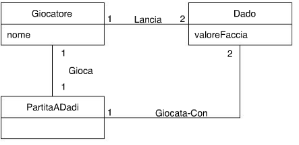
\includegraphics[scale=0.7]{images/Dadi.png}
\end{center}

\subsubsection{Assegnare responsabilità agli oggetti e 
disegnare diagrammi di interazione: \fancyglitter{responsabilità e collaborazioni}.}

\begin{center}
    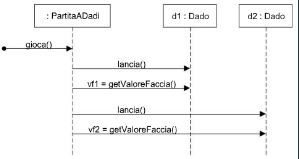
\includegraphics[scale = 0.7]{images/Dadi2.png}
\end{center}

\subsubsection{Definizione dei diagrammi delle classi di progetto.}

\begin{center}
    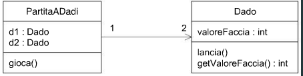
\includegraphics[scale=0.7]{images/Dadi 3.png}
\end{center}

}
\subsubsection{}
L'analisi dei requisiti e l'OOA/D vanno svolte nel contesto di un processo di sviluppo:

\begin{itemize}
    \item [$\Rightarrow$] Sviluppo iteratuivo;
    \item [$\Rightarrow$] Approccio agile;
    \item [$\Rightarrow$] Unified Process (UP).
\end{itemize}

\nt{ER e UML non sono pienamente adatti a possibili incrementi.}
\pagebreak

\subsection{UML}

\dfn{UML}{UML è un linguaggio \newfancyglitter{visuale} per la specifica,
la costruzione e la documentazione degli elaborati di un sistema software.

UML è uno standard per la notazione di diagrammi per disegnare o rappresentare
figure relative al software (specialmente OO).}
\subsubsection{}
UML è un \textit{abbozzo} o un \textit{progetto} per aiutare la comprensione nei team di sviluppo.
Il termine abbozzo indica che può essere soggetto a correzzione, ma se non ci 
sono feedback a tal proposito deve essere trattato come un dizionario.

\subsubsection{Uso di UML:}

\begin{itemize}
    \item [$\Rightarrow$] Punto di vista \fancyglitter{concettuale}: modello 
    di dominio, per visualizzare concetti del mondo reale;
    \item [$\Rightarrow$] Punto di vista \fancyglitter{software}: diagramma
    delle classi di progetto, utilizzata per visualizzare elementi software.
\end{itemize}

\subsubsection{Brevi note storiche:}

\begin{itemize}
    \item [$\Rightarrow$] Anni '60 e '70: nascita dei linguaggi OO (Simula e Smalltalk);
    \item [$\Rightarrow$] 1988: Bertrand Meyer, "Object-Oriented Software";
    \item [$\Rightarrow$] 1991: Jim Rumbaugh, "Object-Oriented Modelling and Design" (OOA/D);
    \item [$\Rightarrow$] 1991, Grady Booch, "Object-Oriented Software Engineering" (OOA/D e Casi d'Uso);
    \item [$\Rightarrow$] 1994, Rumbaugh e Booch fanno le prime proposte di UML;
    \item [$\Rightarrow$] Rational Corporation fondata dai "tre amigos" (Jacobson, Booch e Rumbaugh);
    \item [$\Rightarrow$] 1997 UML 1;
    \item [$\Rightarrow$] 2004 UML 2 (usato attualmente).
\end{itemize}

\section{Unified Process}

\dfn{Unified Process}{
    Unified Process è un processo iterativo ed evolutivo (incrementale)
    per lo sviluppo del software per la costruzione di sistemi orientati agli oggetti.
    Le iterazioni iniziali sono guidate dal \newfancyglitter{rischio}, dal
    \newfancyglitter{cliente} e dall'\newfancyglitter{architettura}.
}

\qs{}{Cosa c'è in UP?}

\begin{itemize}
    \item [$\Rightarrow$] Un'organizzazione del piano di progetto
    per fasi sequenziali;
    \item [$\Rightarrow$] Indicazioni sulle attività da svolgere nell'ambito
    di discipline e sulle loro inter-relazioni;
    \item [$\Rightarrow$] Un insieme di ruoli predefiniti;
    \item [$\Rightarrow$] Un insieme di artefatti da produrre.
\end{itemize}

\subsubsection{Un progetto UP è organizzato in 4 fasi:}

\begin{itemize}
    \item [$\Rightarrow$] \fancyglitter{Ideazione} (inception): visione approssimativa, studio economico, portata, stime approssimative di costi e tempi. \textbf{\underline{Milestone}:} \newfancyglitter{Obiettivi};
    \item [$\Rightarrow$] \fancyglitter{Elaborazione} (elaboration): visione raffinata, implementazione iterativa del nucleo dell'architettura, risoluzione dei rischi maggiori, identificazione della maggior parte dei requisiti e della portata, stime più realistiche sulle loro inter-relazioni. \textbf{\underline{Milestone}:} \newfancyglitter{Architetturale};  
    \item [$\Rightarrow$] \fancyglitter{Costruzione} (construction): implementazione iterativa degli elementi rimanenti, più facili e a rischio minore, preparazione al rilascio. \textbf{\underline{Milestone}:} \newfancyglitter{Capacità operazionale};
    \item [$\Rightarrow$] \fancyglitter{Transizione} (transition): beta test, rilascio. \textbf{\underline{Milestone}:} \newfancyglitter{Rilascio prodotto}.
\end{itemize}

\begin{center}
    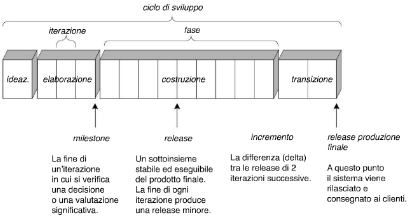
\includegraphics[scale = 1]{images/UP.png}
\end{center}

\nt{
    \begin{itemize}
        \item [$\Rightarrow$] L'Ideazione non è una fase di requisiti, ma di fattibilità;
        \item [$\Rightarrow$] L'Elaborazione non è una fase di requisiti o di progettazione, ma una fase in cui 
        si implementa in modo iterativo l'architettura del sistema e vengono ridotti i rischi maggiori.
    \end{itemize}
}

\subsection{Le discipline}

\dfn{Discipline}{
    Una disciplina è un insieme di attività e dei relativi \newfancyglitter{elaborati}
    in una determinata area, come le attività relative all'analisi dei requisiti. 
}

\cor{Elaborato}{
    Un elaborato (artefatto o work product) è il termine generico che indica un qualsiasi prodotto di lavoro: codice, schemi di basi di dati, 
    documenti di testo, diagrammi, modelli, etc.
}

\subsubsection{Discipline ingegneristiche di UP:}

\begin{itemize}
    \item [$\Rightarrow$] \fancyglitter{Modellazione del business}: attività che 
    modellano il dominio del problema e il suo ambito;
    \item [$\Rightarrow$] \fancyglitter{Requisiti}: attività di raccolra dei requisiti;
    \item [$\Rightarrow$] \fancyglitter{Progettazione} (analysis and design): attività di analisi dei requisiti
    e progetto architetturale;
    \item [$\Rightarrow$] \fancyglitter{Implementazione}: attività di progetto dettagliato e codifica del sistema, test sui componenti;
    \item [$\Rightarrow$] \fancyglitter{Test}: attività di controllo di qualità, test di integrazione e di sistema;
    \item [$\Rightarrow$] \fancyglitter{Rilascio}: attività di consegna e messa in opera.
\end{itemize}

\subsubsection{Discipline di supporto di UP:}

\begin{itemize}
    \item [$\Rightarrow$] \fancyglitter{Gestione delle configurazioni e del cambiamento}: attività di manutenzione durante il progetto;
    \item [$\Rightarrow$] \fancyglitter{Gestione progetto}: attività di pianificazione e governo del progetto;
    \item [$\Rightarrow$] \fancyglitter{Infrastruttura} (enviroment): attività che supportano il team di progetto, riguardo ai processi e strumenti utilizzati.
\end{itemize}

\nt{Nonostante le fasi siano \newfancyglitter{sequenziali}, le discipline non lo sono (perchè si eseguono in ogni iterazione).
Il numero di iterazioni dipende dal Project Manager.}

\subsubsection{Uso di UML in UP:}

\begin{itemize}
    \item [$\Rightarrow$] UP usa solo UML come linguaggio di modellazione;
    \item [$\Rightarrow$] I diagrammi UML si usano con variabilità, bisogna \newfancyglitter{personalizzare} UP;
    \item [$\Rightarrow$] I diagrammi si usano in UP seguendo le iterazioni e gli incrementi;
    \item [$\Rightarrow$] UP dice \newfancyglitter{quando} usare un diagramma;
    \item [$\Rightarrow$] In UP quasi tutto è \newfancyglitter{opzionale} eccetto che lo sviluppo iterativo e guidato dal rischio, la verifica continua della qualità e il codice;
    \item [$\Rightarrow$] La scelta delle pratiche e degli artefatti UP si riassume in un documento (\newfancyglitter{scenario di sviluppo}).
\end{itemize}

\subsection{Che cosa sono i requisiti?}

\dfn{Requisito}{
    Un requisito è una \newfancyglitter{capacità} o una condizione a cui il sistema deve essere \newfancyglitter{conforme}.
}

\cor{Sorgenti dei requisiti}{
    I requisiti derivano da richieste degli utenti del sistema per risolvere dei problemi e raggiungere degli obiettivi.
    Possono essere:
    \begin{itemize}
        \item [$\Rightarrow$] \fancyglitter{Requisiti funzionali}: descrivono il comportamento del sistema in termini di funzionalità offerte;
        \item [$\Rightarrow$] \fancyglitter{Requisiti non funzionali}: le proprietà del sistema nel suo complesso (sicurezza, prestazioni, etc.).
    \end{itemize}
}

\nt{
    In UP bisogna gestire i requisiti: si utilizza un approccio sistematico
    per trovare, documentare, organizza e tracciare i \underline{requisiti che cambiano}
    di un sistema. Si inizia a programmare quando sono stati specificati il 10\% o il 20\%
    dei requisiti significativi.
}

\subsubsection{Acquisizione sistematica dei requisiti:}

\begin{itemize}
    \item [$\Rightarrow$] Scrivere i Casi d'Uso con i clienti;
    \item [$\Rightarrow$] Workshop dei requisiti con sviluppatori e clienti;
    \item [$\Rightarrow$] Gruppi di lavoro con rappresentanti dei clienti;
    \item [$\Rightarrow$] Dimostrazione ai clienti dei risultati di ciascuna iterazione, per favorire un feedback.
\end{itemize}

\subsubsection{Modello FURPS+:}

\begin{itemize}
    \item [$\Rightarrow$] \fancyglitter{Funzionali} (F): requisiti funzionali e di sicurezza;
    \item [$\Rightarrow$] \fancyglitter{Usabilità} (U): facilità d'uso del sistema;
    \item [$\Rightarrow$] \fancyglitter{Affidabilità} (R - Reliability): disponibilità del sistema, capacità di tollerare guasti o di essere ripristinato;
    \item [$\Rightarrow$] \fancyglitter{Prestazioni} (P): tempi di risposta, throughput, capacità e uso delle risorse;
    \item [$\Rightarrow$] \fancyglitter{Sostenibilità} (S): facilità di modifica per riparazioni e miglioramenti, adattabilità, manutenibilità, localizzazione, configurazione, compatibilità;
    \item [$\Rightarrow$] \fancyglitter{+}: vincoli di progetto, interoperabilità, operazionali, fisici, legali, etc.
\end{itemize}

\subsubsection{Elaborati:}

\begin{itemize}
    \item [$\Rightarrow$] \fancyglitter{Modello dei Casi d'Uso}: scenari tipi dell'utilizzo di un sistema;
    \item [$\Rightarrow$] \fancyglitter{Specifiche supplementari}: ciò che non rientra nei Casi d'Uso, requisiti non funzionali o funzionali non esprimibili attraverso i Casi d'Uso;
    \item [$\Rightarrow$] \fancyglitter{Glossario}: termini significativi, dizionario dei dati;
    \item [$\Rightarrow$] \fancyglitter{Visione}: riassume i requisiti di alto livello, un documento sintetico per apprendere rapidamente le idee principali del progetto;
    \item [$\Rightarrow$] \fancyglitter{Regole di Business}: regole di dominio, i requisiti o le politiche che trascendono un unico progetto software e a cui un sistema deve conformarsi.
\end{itemize}

\section{Ideazione}

\qs{}{Che cos'è l'ideazione?}

\paragraph{Risposta:} l'ideazione permette di stabilire una visione completa
e la portata del progetto (\newfancyglitter{studio di fattibilità}).

\subsubsection{Durante l'ideazione:}

\begin{itemize}
    \item [$\Rightarrow$] Si analizzano il 10\% dei Casi d'Uso;
    \item [$\Rightarrow$] Si analizzano i requisiti non funzionali più importanti;
    \item [$\Rightarrow$] Si realizza una stima dei costi;
    \item [$\Rightarrow$] Si prepara l'ambiente di sviluppo;
    \item [$\Rightarrow$] \newfancyglitter{Durata:} breve.
\end{itemize}

\nt{Lo scopo dell'Ideazione \underline{non} è di raccogliere tutti i requisiti, né di generare
una stima o un piano di progetto affidabile.
Durante l'ideazione si cerca di capire se il progetto è fattibile e se ha senso.}

\definecolor{dkgreen}{rgb}{0, 0.5, 0}
\definecolor{mgray}{rgb}{0.9, 0.9, 0.9}
\begin{center}
    \begin{tabular}{ || >{\columncolor{mgray}}p{8cm} | >{\columncolor{GreenPastel}}p{8cm} ||}
    \hline\hline
        \rowcolor{lightgray}
    \textbf{Elaborato}& \textbf{\textcolor{dkgreen}{Commento}}\\ \hline
    \hline
        Visione e studio economico & Descrive obiettivi e vincoli di alto livello, fornisce un sommario del progetto.\\ \hline

        Modello dei Casi d'Uso & Descrive i requisiti funzionali del sistema. Vengono identificati i nomi della maggior parte dei Casi d'Uso.\\ \hline

        Specifiche supplementari & Descrive i requisiti non funzionali e i requisiti funzionali non esprimibili attraverso i Casi d'Uso.\\ \hline

        Glossario & Definisce i termini significativi del dominio.\\ \hline

        Lista dei Rischi e Piano di Gestione dei Rischi & Identifica i rischi principali e come affrontarli.\\ \hline

        Prototipi e proof of concept & Dimostrano la fattibilità tecnica e la comprensione dei requisiti.\\ \hline

        Piano dell'Iterazione & Fornisce una descrizione di cosa fare nella prima iterazione dell'elaborazione.\\ \hline

        Piano delle Fasi e Piano di Sviluppo del Software & Ipotesi (poco precise) riguardo la fase di elaborazione.\\ \hline 
    
        Scenario di Sviluppo & Descrive le pratiche e gli artefatti UP da usare.\\ \hline
    
        \hline

    \end{tabular}
\end{center}

\subsection{Artefatti nell'Ideazione}

\qs{}{La documentazione non è troppa?}

\paragraph{Risposta:} lo scopo della documentazione non è nel documento in sè, ma nel pensare:

\begin{itemize}
    \item [$\Rightarrow$] gli artefatti sono quelli che aggiungono valore;
    \item [$\Rightarrow$] sono parzialmente completati;
    \item [$\Rightarrow$] sono preliminari e approssimativi.
\end{itemize}

\nt{Nessun documento è definitivo.}

\dfn{Specifiche supplementari}{
    Le \newfancyglitter{specifiche supplementari} raccolgono altri requisiti,
    informazioni e vincoli che non sono espressi nei Casi d'Uso o nel Glossario. 
    Si deve mettere anche la cronologia delle versioni.
}

\subsection{Tipologie di documenti}

\dfn{Visione}{
    Il documento \newfancyglitter{Visione} riassume alcune informazioni contenute nel modello dei Casi d'Uso e 
    nelle Specifiche supplementari. Inoltre descrive brevemente il progetto ai partecipanti per stabilire una
    visione comune.
    
    \begin{itemize}
        \item [$\Rightarrow$] Obiettivi e problemi fondamentali ad alto livello\footnote{Soprattutto per i requisiti non funzionali};
        \item [$\Rightarrow$] Riepilogo delle caratteristiche di sistema.
    \end{itemize}
}

\nt{Spesso è utile iniziare da un Glossario.}

\dfn{Glossario e dizionario dei dati}{
    Il \newfancyglitter{Glossario} è un documento che definisce i termini significativi del dominio e le relazioni tra di
    essi. Si devono eliminare eventuali discrepanze per ridurre problemi di comunicazione e di ambiguità.

    In UP il Glossario svolge anche il ruolo di \newfancyglitter{dizionario dei dati}:
    un documento di dati che si riferiscono ad altri dati\footnote{Metadati.}, per esempio le regole di validazione.
}

\cor{Regole di dominio}{
    Le \newfancyglitter{regole di dominio} (o regole di Business\footnote{Viste in "Basi di dati".}) stabiliscono
    come può funzionare un dominio o un business.

}


\section{Casi d'Uso}



\section{Elaborazione}

\section{Modello di Dominio}

\section{Diagrammi di sequenza del sistema (DSS)}

\section{Contratti}

\definecolor{chaptergrey}{rgb}{1,0.75,0}
\ifnum\layout=2 
    \fancyhf{}      
    \renewcommand{\headrulewidth}{0pt}
    \renewcommand{\chaptermark}[1]{\markboth{#1}{}}

    \fancyhead[LE]{\nouppercase{\textbf{\textcolor{chaptergrey}{\chaptername}}~ \thechapter~ |~ \leftmark}}
    \fancyhead[RO]{\nouppercase{ \rightmark}}
    \fancyfoot[LE,RO]{\thepage}
    \fancypagestyle{plain}{         
    \fancyhf{}
    \fancyfoot[LE,RO]{\thepage}}    
 \else          
    \renewcommand{\headrulewidth}{0pt}
    \fancyhf{}                  
    \fancyhead[C]{\nouppercase{ \leftmark}}
    \fancyfoot[C]{\thepage}
\fi

\chapter{Architettura del software}

\section{Architettura logica}

\dfn{Architettura}{
    La progettazione OO è  basata su diversi strati architetturali,
    come uno strati UI, uno strato di logica applicativa (o "del dominio") e così via.
}

\nt{L'architettura può essere mostrata sotto forma di diagrammi UML.}

\ex{Package UML}{
    \begin{center}
        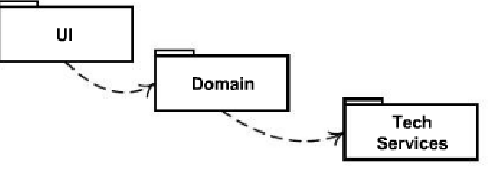
\includegraphics[scale=0.5]{images/PackageUML.png}
    \end{center}
}

\dfn{Architettura logica}{
    L'\newfancyglitter{architettura logica} di un sistema
    software è la macro-organizzazione su larga scala delle 
    classi in package (o namespace), sottoinsiemi e strati.
}

\nt{Non vengono prese decisioni su come gli elementi sono distribuiti
sui processi o sui vari computer fisici di una rete (\fancyglitter{platform independent architecture}).}

\cor{Layer (o Strato)}{
    Un layer è un gruppo di classi software, packages, sottosistemi con responsabilità
    condivisa su un aspetto importante del sistema.
}

\subsubsection{Gli strati comprendono:}

\begin{itemize}
    \item [$\Rightarrow$] \fancyglitter{UI (User Interface)}: strato che si occupa dell'interazione con l'utente;
    \item [$\Rightarrow$] \fancyglitter{Application logic} (o "domain object"): oggetti software che rappresentano concetti di dominio;
    \item [$\Rightarrow$] \fancyglitter{Technical services}: oggetti e sottosistemi che forniscono servizi tecnici (es. persistenza, sicurezza, ecc.);
\end{itemize}

\subsubsection{Rappresentazioni di strati:}
    \begin{figure}[!h]
        \centering
        \subfloat[Packeges UML]{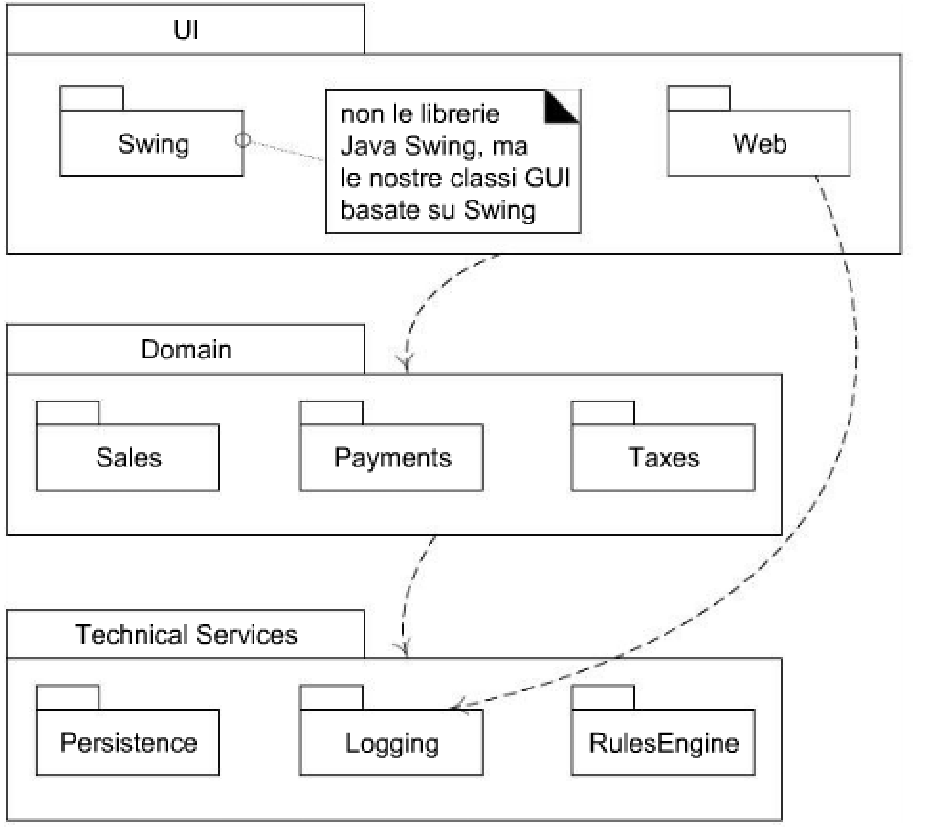
\includegraphics[scale = 0.25]{images/UMLPackage.png}} 
        \subfloat[Relativo codice]{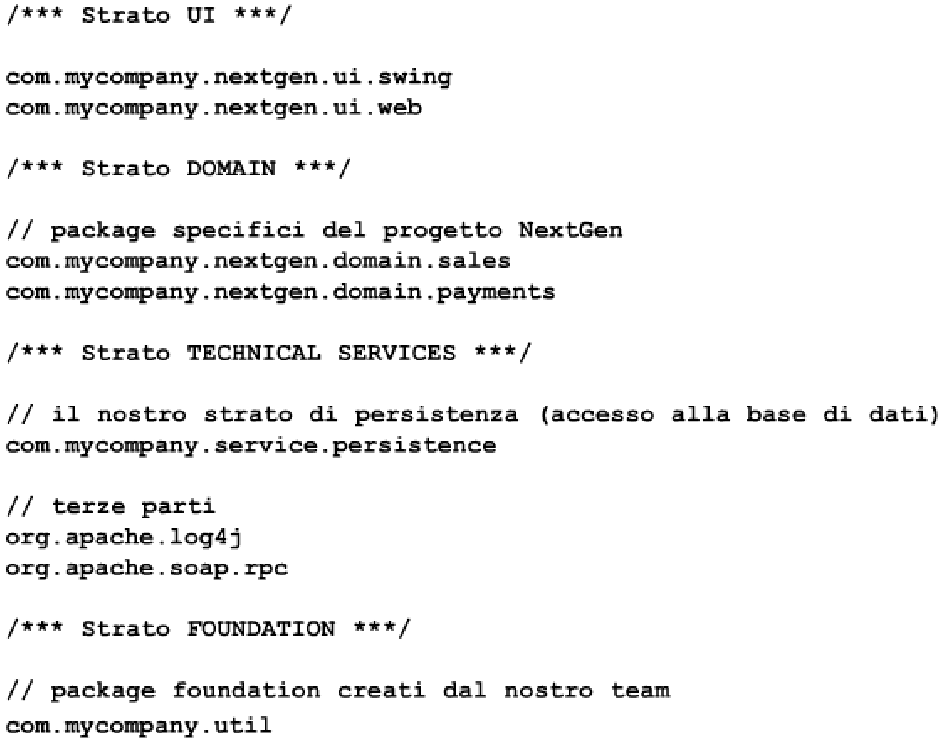
\includegraphics[scale = 0.25]{images/PackageCode.png}}
    \end{figure}

\dfn{Architettura a strati}{
    L'obiettivo di un'\newfancyglitter{architettura a strati} è la suddivisione di un sistema complesso
    in un insieme di elementi software che possano essere sviluppati e modificati in modo indipendente.
}

\cor{Separation of concerns}{
    La separazione degli interessi:

    \begin{itemize}
        \item [$\Rightarrow$] Riduce l'accoppiamento e le dipendenze;
        \item [$\Rightarrow$] Aumenta la possibilità di riuso;
        \item [$\Rightarrow$] Facilita la manutenzione e l'evoluzione del sistema;
        \item [$\Rightarrow$] Aumenta la chiarezza.
    \end{itemize}
}

\cor{Alta coesione}{
    In uno strato le responsabilità degli oggetti devono essere fortemente
    collegate tra loro, ma non essere mischiate con quelle di altri strati.
}

\nt{Questi due principi verranno ripresi in GRASP, vedi capitolo \ref{GRASP}.}

\pagebreak

\ex{Architettura a strati}{
    \begin{center}
        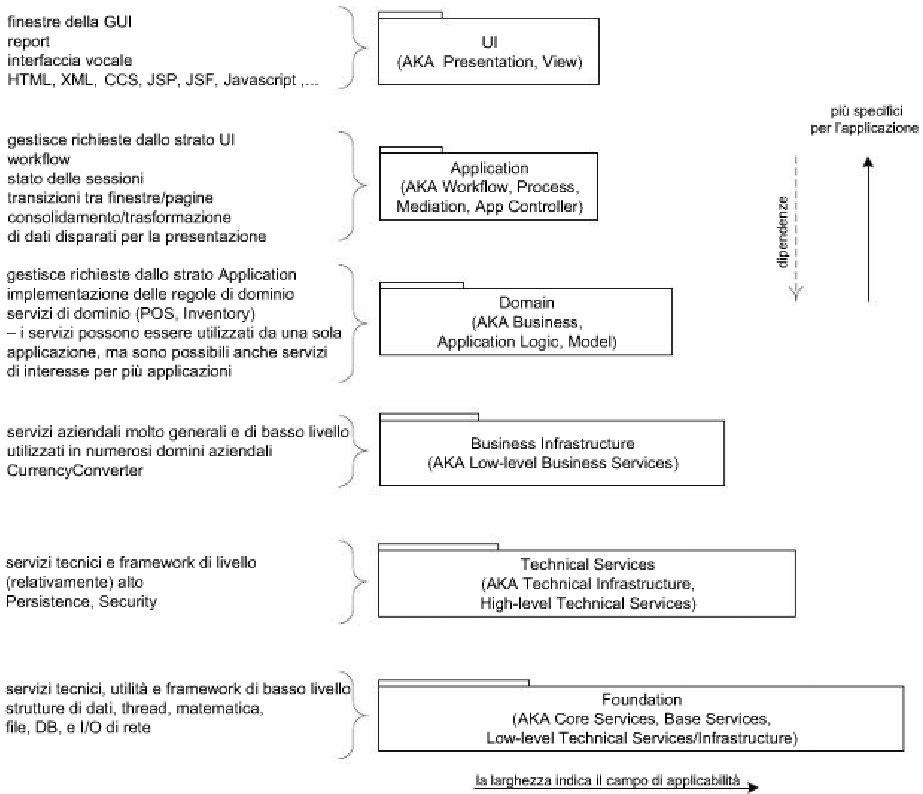
\includegraphics[scale=0.45]{images/Architettura a strati.png}
    \end{center}

}


\section{Strato del dominio}

\qs{}{Come va progettata la logica applicativa con gli oggetti?}

\paragraph{Risposta:} Si creano oggetti software con nomi e informazioni simili
al Dominio del mondo reale e assegnare a essi le responsabilità della logica applicativa.

\dfn{Oggetto del Dominio}{
    Un \newfancyglitter{oggetto del dominio} è un oggetto software che rappresenta un concetto del dominio del problema.

    Ha una logica applicativa o di business correlata.
}

\nt{Ispirandosi al Modello del Dominio si ha un basso salto rappresentazionale che
rende più facile e veloce l'implementazione.}

\ex{Strato di Dominio e Modello di Dominio}{

    \begin{center}
        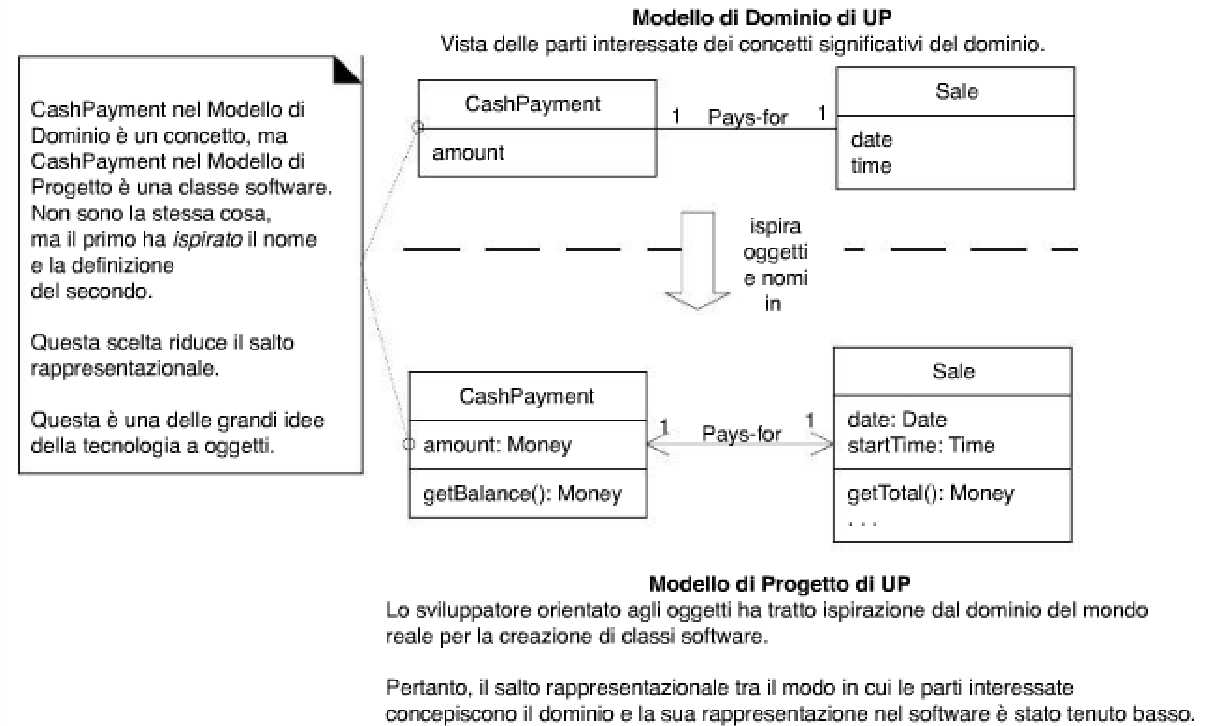
\includegraphics[scale=0.35]{images/Modello.png}
    \end{center}
}

\ex{Strati e Partizioni}{
    \begin{center}
        \includegraphics[scale=0.35]{images/Strati e Partizioni.png}
    \end{center}
}

\section{Separazione Modello-Vista}

\dfn{Principio di separazione Modello-Vista}{
    \begin{itemize}
        \item [\textcolor{red}{\XSolidBrush}] Non relazionare o accoppiare oggetti non UI con oggetti UI;
        \item [\textcolor{red}{\XSolidBrush}] Non incapsulare la logica applicativa in metodi UI;
        \item [\textcolor{green}{\Checkmark}] Le finestre appartengono a una specifica applicazione, mentre
        gli oggetti non UI possono venire riutilizzati in nuove applicazioni o associati a nuove interfacce;
        \item [\textcolor{green}{\Checkmark}] Gli oggetti UI inizializzano elementi UI, ricevono eventi UI e
        delegano le richieste della logica dell'applicazione agli oggetti non UI.
    \end{itemize}
}

\nt{
    \begin{itemize}
        \item [$\Rightarrow$] Il Modello è lo strato degli oggetti del dominio;
        \item [$\Rightarrow$] La Vista è lo strato UI.
    \end{itemize}

    Questo principio è alla base del pattern MVC\footnote{Visto nel corso "Programmazione III".}.
}

\subsubsection{Ulteriori considerazioni:}

\begin{itemize}
    \item [$\Rightarrow$] Le classi di dominio incapsulano le informazioni e il comportamento della logica applicativa;
    \item [$\Rightarrow$] Le classi della vista sono leggere, sono responsabili dell'inpute e dell'output, ma non mantengono dati.
\end{itemize}

\subsubsection{Vantaggi:}

\begin{itemize}
    \item [$\Rightarrow$] Favorire la definizione coesa dei modelli;
    \item [$\Rightarrow$] Consentire lo sviluppo separaro;
    \item [$\Rightarrow$] Minimizzare l'impatto sullo strato del dominio;
    \item [$\Rightarrow$] Consentire di connettere facilmente nuove viste;
    \item [$\Rightarrow$] Consentire l'esecuzione dello strato di modello indipendentemente dallo strato UI;
    \item [$\Rightarrow$] Consentire un \textit{porting} facile dello strato di modello a un altro framework UI.
\end{itemize}

\ex{SSD e UI}{
    \begin{center}
        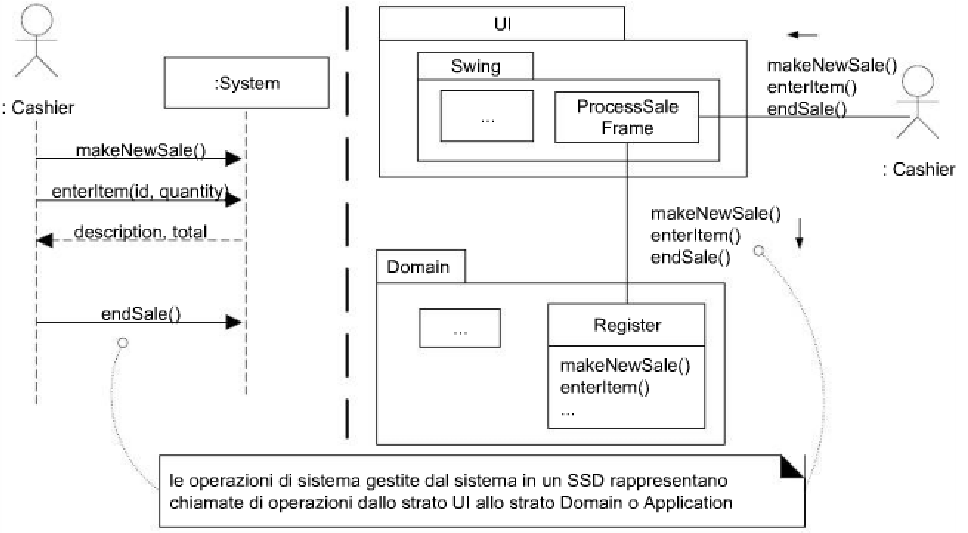
\includegraphics[scale=0.3]{images/SSD e UI.png}
    \end{center}
}
\definecolor{chaptergrey}{rgb}{1,0.75,0.8}
\ifnum\layout=2 
    \fancyhf{}      
    \renewcommand{\headrulewidth}{0pt}
    \renewcommand{\chaptermark}[1]{\markboth{#1}{}}

    \fancyhead[LE]{\nouppercase{\textbf{\textcolor{chaptergrey}{\chaptername}}~ \thechapter~ |~ \leftmark}}
    \fancyhead[RO]{\nouppercase{ \rightmark}}
    \fancyfoot[LE,RO]{\thepage}
    \fancypagestyle{plain}{         
    \fancyhf{}
    \fancyfoot[LE,RO]{\thepage}}    
 \else          
    \renewcommand{\headrulewidth}{0pt}
    \fancyhf{}                  
    \fancyhead[C]{\nouppercase{ \leftmark}}
    \fancyfoot[C]{\thepage}
\fi

\chapter{Diagrammi di interazione e di classe UML}

\section{Verso la progettazione a oggetti}

\qs{}{Come si progetta a oggetti?}

\begin{itemize}
    \item [$\Rightarrow$] \fancyglitter{Codifica}: si progetta mentre
    si codifica;
    \item [$\Rightarrow$] \fancyglitter{Disegno, poi codifica}: si
    disegnano i diagrammi UML e poi si codifica;
    \item [$\Rightarrow$] \fancyglitter{Solo disegno}: si disegnano i
    diagrammi UML e lo strumento genera ogni cosa da essi.
\end{itemize}

\nt{Solitamente si sceglie di disegnare e poi codificare.}

\subsection{Modellazione dinamica e statica}

\dfn{Modelli dinamici}{Rappresentano il comportamento del sistema,
la collaborazione tra oggetti per realizzare dei Casi d'Uso. Di solito
si utilizzano i diagrammi di interazione UML.}

\dfn{Modelli statici}{
    Servono per definire package, nomi delle classi, attributi e
    firme di operazioni. Di solito si utilizzano i diagrammi delle
    classi UML.
}

\nt{Solitamente si creano in parallelo sia i modelli dinamici che
statici.}
\pagebreak
\ex{Modelli statici e dinamici}{
    \begin{center}
        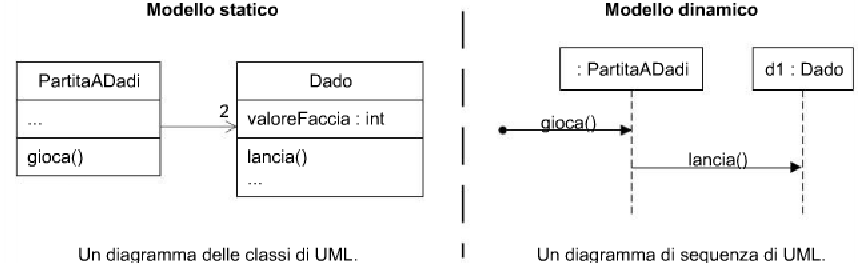
\includegraphics[scale=0.45]{images/Modelli statici e dinamici.png}
    \end{center}
}

\begin{itemize}
    \item [$\Rightarrow$] La maggior parte del lavoro utile e difficile
    avviene nel disegno dei diagrammi di interazione (o di sequenza);
    \item [$\Rightarrow$] Durante la modellazione dinamica si pensa
    a quali oggetti devono esistere e a come collaborano tra loro;
    \item [$\Rightarrow$] Per la modellazione dinamica si fa riferimento
    ai principi GRASP\footnote{Vedi capitolo \ref{GRASP}.}.
\end{itemize}

\subsubsection{Le domande che ci si deve porre sono:}

\begin{itemize}
    \item [$\Rightarrow$] \fancyglitter{Quali} sono le responsabilità
    dell'oggetto?
    \item [$\Rightarrow$] \fancyglitter{Chi} collabora con chi?
    \item [$\Rightarrow$] \fancyglitter{Quali} design pattern devono essere applicati?
\end{itemize}

\subsubsection{La progettazione a oggetti richiede la conoscenza di:}

\begin{itemize}
    \item [$\Rightarrow$] \fancyglitter{Design pattern};
    \item [$\Rightarrow$] \fancyglitter{Principi di assegnazione delle responsabilità}.
\end{itemize}

\section{Diagrammi di interazione}

\dfn{Interazione}{
    Un'\newfancyglitter{interazione} è una specifica di come alcuni
    oggetti si scambiano messaggi nel tempo per eseguire un compito nell'ambito
    di un certo contesto.
}

\nt{Il termine diagramma di interazione si riferisce a due tipi di diagrammi:
\begin{itemize}
    \item [$\Rightarrow$] \fancyglitter{Diagrammi di sequenza};
    \item [$\Rightarrow$] \fancyglitter{Diagrammi di comunicazione}.

\end{itemize}

In questo corso ci concentreremo sui diagrammi di sequenza.
}

\subsubsection{Caratteristiche dei diagrammi di sequenza:}

\begin{itemize}
    \item [$\Rightarrow$] Un'\fancyglitter{interazione} è motivata dalla necessità
    di eseguire un \fancyglitter{compito};
    \item [$\Rightarrow$] Un \fancyglitter{compito} è rappresentato da un 
    \fancyglitter{messaggio} che dà inizio all'interazione (messaggio trovato);
    \item [$\Rightarrow$] Il \fancyglitter{messaggio} è inviato a un oggetto designato
    come \fancyglitter{responsabile} del compito;
    \item [$\Rightarrow$] L'oggetto \fancyglitter{responsabile} collabora con
    altri oggetti (\fancyglitter{partecipanti}) per eseguire il compito;
    \item [$\Rightarrow$] Ciascun \fancyglitter{partecipante} svolge un proprio
    \fancyglitter{ruolo} nell'interazione;
    \item [$\Rightarrow$] La \fancyglitter{collaborazione} avviene mediante 
    \fancyglitter{messaggi} scambiati tra gli oggetti;
    \item [$\Rightarrow$] Ciascun messaggio è una richiesta che un oggetto fa a un altro
    oggetto di eseguire un'\fancyglitter{operazione}.
\end{itemize}

\subsubsection{Vantaggi e svantaggi dei diagrammi di sequenza:}

\begin{itemize}
    \item [\textcolor{green}{\checkmark}] Mostrano chiaramente la sequenza 
    dell'ordinamento temporale dei messaggi.
    \item [\textcolor{red}{\XSolidBrush}] Costringono a estendersi verso destra
    quando si aggiungono nuovi oggetti.
\end{itemize}

\ex{Diagrammi di sequenza}{
    \begin{center}
        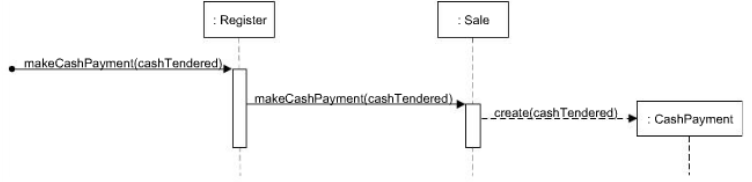
\includegraphics[scale=0.45]{images/Diagramma di sequenza.png}
    \end{center}
}

\subsection{Diagrammi di sequenza del design (DSD)}

\dfn{Design Sequence Diagram (DSD)}{
    Un \newfancyglitter{diagramma di sequenza} di progetto è un diagramma
    di sequenza utilizzato da un punto di vista software o di progetto.
}

\nt{In UP l'insieme di tutti i DSD fa parte del modello di progetto.}

\ex{Notazione di DSD: partecipanti}{
    \begin{center}
        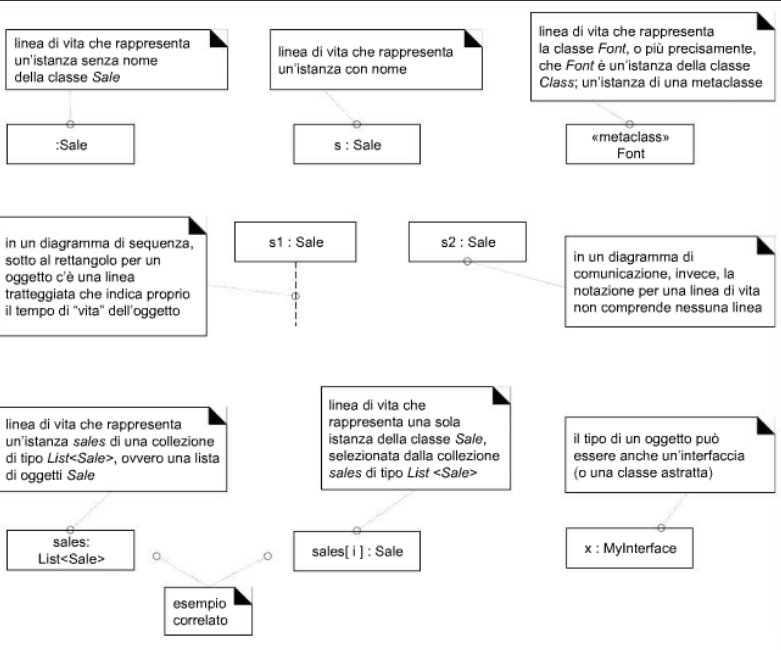
\includegraphics[scale=0.35]{images/Notazione di DSD.png}
    \end{center}
}

\dfn{Singleton}{
    Un \newfancyglitter{singleton} è un pattern nel quale da una classe viene istanziata una sola istanza.
}

\ex{Notazione di DSD: singleton}{
    \begin{center}
        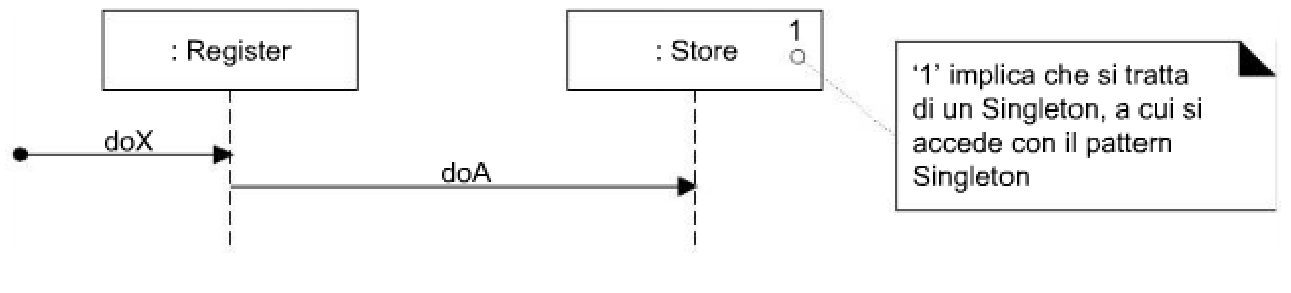
\includegraphics[scale=0.25]{images/Singleton.png}
    \end{center}
}



\section{Diagrammi delle classi}




\definecolor{chaptergrey}{rgb}{0,0.13, 0.38}
\ifnum\layout=2 
    \fancyhf{}      
    \renewcommand{\headrulewidth}{0pt}
    \renewcommand{\chaptermark}[1]{\markboth{#1}{}}

    \fancyhead[LE]{\nouppercase{\textbf{\textcolor{chaptergrey}{\chaptername}}~ \thechapter~ |~ \leftmark}}
    \fancyhead[RO]{\nouppercase{ \rightmark}}
    \fancyfoot[LE,RO]{\thepage}
    \fancypagestyle{plain}{         
    \fancyhf{}
    \fancyfoot[LE,RO]{\thepage}}    
 \else          
    \renewcommand{\headrulewidth}{0pt}
    \fancyhf{}                  
    \fancyhead[C]{\nouppercase{ \leftmark}}
    \fancyfoot[C]{\thepage}
\fi

\chapter{Pattern GRASP}
\label{GRASP}

\section{Responsability-Driven Development}

\dfn{Responsability-Driven Development (RDD)}{
    L'approccio complessivo al fare la modellazione per la programmazione
    OO si basa sulla metafore della \newfancyglitter{progettazione guidata dalle responsabilità} (RDD),
    che è un modo di pensare a come assegnare le responsabilità agli oggetti
    che collaborano.
}

\cor{responsabilità}{
    Per responsabilità si intende un'astrazione di ciò che fa o rappresenta
    un oggetto o un componente software. Le responsabilità sono di due tipi:
    \begin{itemize}
        \item [$\Rightarrow$] Di fare;
        \item [$\Rightarrow$] Di conoscere.
    \end{itemize}
}

\nt{In UML la responsabilità è un \fancyglitter{contratto} o 
un \fancyglitter{obbligo} di un oggetto.}

\subsection{Tipi di responsabilità}

\subsubsection{Le responsabilità di fare comprendono:}

\begin{itemize}
    \item [\textcolor{green}{\checkmark}] un oggetto fa qualcosa per sè stesso;
    \item [\textcolor{green}{\checkmark}] un oggetto chiede ad altri oggetti di fare qualcosa;
    \item [\textcolor{green}{\checkmark}] un oggetto controlla e coordina le attività di altri oggetti.
\end{itemize}

\subsubsection{Le responsabilità di conoscere comprendono:}

\begin{itemize}
    \item [\textcolor{green}{\checkmark}] un oggetto conosce i propri dati privati;
    \item [\textcolor{green}{\checkmark}] un oggetto conosce le informazioni di oggetti correlati;
    \item [\textcolor{green}{\checkmark}] un oggetto conosce informazioni che può ricavare o calcolare.
\end{itemize}

\ex{Responsabilità}{
    Si può dichiarare che la classe \textit{Sale} è responsabile di:
    \begin{itemize}
        \item [$\Rightarrow$] creare oggetti \textit{SaleLineItems} (\fancyglitter{responsabilità di fare});
        \item [$\Rightarrow$] conoscere il suo totale (\fancyglitter{responsabilità di conoscere}).
    \end{itemize}
}

\nt{Le responsabilità più grandi coinvolgono centinaia di classi e di metodi, 
mentre le responsabilità più piccole coinvolgono poche classi e pochi metodi (anche solo un metodo).}

\subsubsection{La progettazione guidata dalle responsabilità:}

\begin{enumerate}
    \item Identificare le responsabilità, considerandole una alla volta;
    \item Decidere a quali oggetti assegnare le responsabilità. Potrebbero
    essere oggetti già esistenti o nuovi oggetti;
    \item Capire come fa un oggetto a soddisfare le proprie responsabilità. Potrebbe 
    farlo da solo o collaborando con altri oggetti.
\end{enumerate}


\section{General Responsibility Assignment Software Patterns}


\dfn{GRASP}{
\newfancyglitter{GRASP} è l'acronimo di General Responsibility Assignment Software Patterns. 
Si tratta di un insieme di linee guida per la progettazione orientata agli oggetti. I pattern GRASP sono dei principi generali che possono essere applicati in modo flessibile e adattato a seconda del contesto. 
Sono un aiuto per acquisire padronanza dell'OOD.
}

\nt{Sono principi di buona programmazione, ma adeguatamente motivati.}

\qs{}{Cosa sono i pattern?}

\dfn{Pattern}{
    I principi e gli idiomi se codificati in un linguaggio strutturato, che descrive il
    \newfancyglitter{problema} e la \newfancyglitter{soluzione} e a cui è assegnato
    un nome, diventano un \newfancyglitter{pattern}.

    Un \newfancyglitter{pattern} è una coppia problema/soluzione ben conosciuta che può
    essere applicata in \newfancyglitter{nuovi contesti} con compromessi, implementazioni, variazioni, etc.
}

\qs{}{Da dove arrivano i pattern?}

\begin{itemize}
    \item [$\Rightarrow$] La nozione di pattern fu introdotta da Christopher Alexander
    nei "pattern architettonici";
    \item [$\Rightarrow$] I pattern software furono introdotti da Kent Beck e sviluppati da
    Beck con Ward Cunningham;
    \item [$\Rightarrow$] Nel 1994 viene pubblicato il libro "Design Patterns" di Erich Gamma, Richard Helm, Ralph Johnson e John Vlissides.
    vengono descritti 23 pattern software, noti come i \newfancyglitter{Gang of Four} (GoF).
\end{itemize}

\dfn{Low Representational Gap (LGR)}{
    Quando si progetta vale \newfancyglitter{LRG}: si cerca di ridurre 
    il divario tra il mondo reale e il mondo del software.
}

\cor{Progettazione modulare}{
    Comprensibilità, modificabilità, impatto nei cambiamenti basso,
    flessibilità, riuso, semplicità sono garantiti dal principio di
    \fancyglitter{progettazione modulare}: il software viene diviso 
    in moduli coesi (High Cohesion) e debolmente accoppiati (Low Coupling).
}

\nt{I pattern High Cohesion e Low Coupling sarebbero sufficienti per garantire
una corretta assegnazione delle responsabilità, ma in pratica sono
difficili da applicare direttamente (perchè sono pattern valutativi).}

\section{I pattern GRASP}

Dei 9 pattern GRASP si andranno ad analizzare solamente:
\begin{itemize}
    \item [$\Rightarrow$] Creator;
    \item [$\Rightarrow$] Information Expert;
    \item [$\Rightarrow$] Low Coupling;
    \item [$\Rightarrow$] Controller;
    \item [$\Rightarrow$] High Cohesion.
\end{itemize}

\subsection{Creator}

\mypattern{Creator - Creatore}{
    \paragraph{Problema:} Chi crea un oggetto A? Chi deve essere responsabile
    della creazione di una nuova istanza di una classe?

    \paragraph{Soluzione:} Assegnare alla classe B la responsabilità di creare un'istanza della classe A 
    se una delle seguenti condizioni è vera:

    \begin{itemize}
        \item [$\Rightarrow$] B \textbf{aggrega} o \textbf{contiene} A;
        \item [$\Rightarrow$] B registra A\footnote{Registrare significa salvare un riferimento.};
        \item [$\Rightarrow$] B utilizza strettamente A;
        \item [$\Rightarrow$] B ha i dati necessari per inizializzare A.
    \end{itemize}
}

\nt{Più condizioni sono vere, meglio è.}
\pagebreak
\ex{Monopoly}{
    \begin{center}
        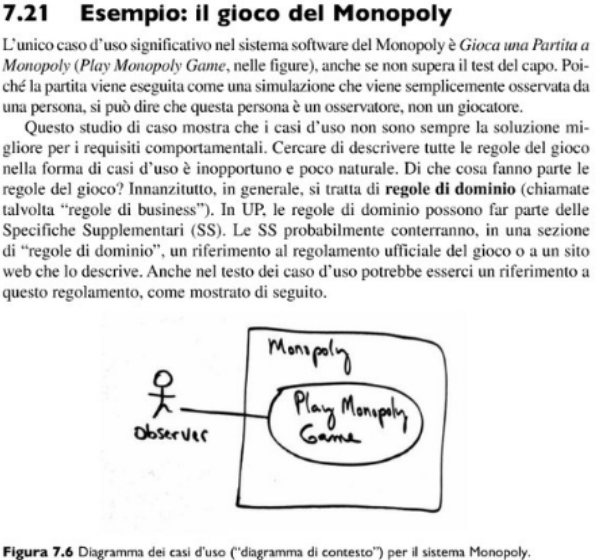
\includegraphics[scale=0.45]{images/Monopoly1.png}
        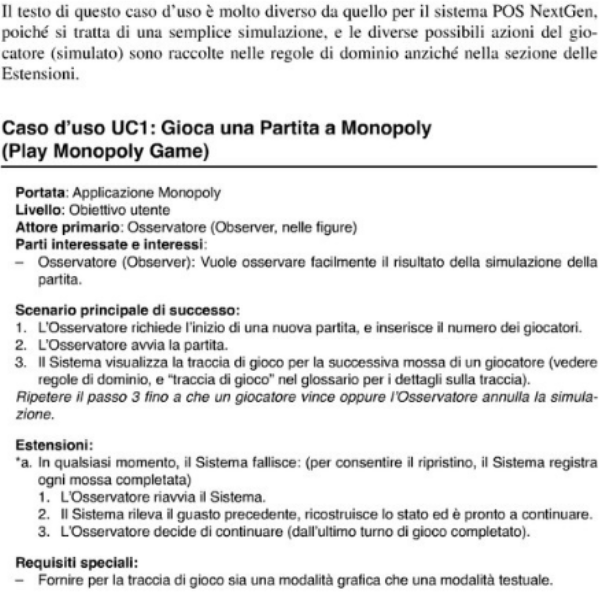
\includegraphics[scale=0.35]{images/Monopoly2.png}
        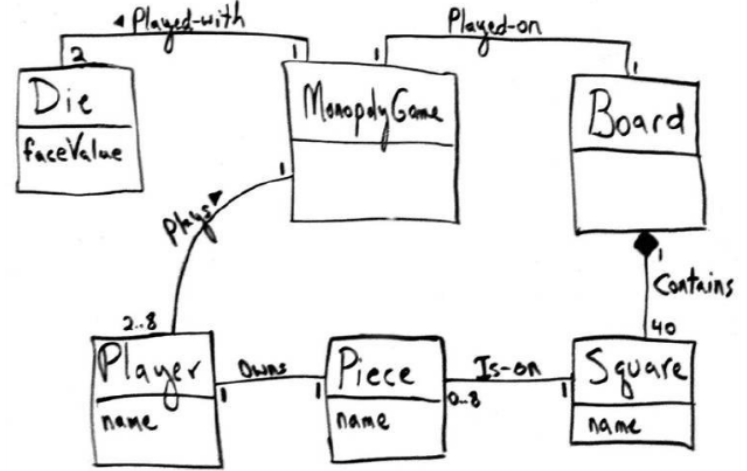
\includegraphics[scale=0.35]{images/Monopoly3.png}
    \end{center}
}

\clm{}{}{
    \begin{itemize}
        \item [$\Rightarrow$] Trovare un creatore che abbia effettivamente bisogno di essere collegato
        a un oggetto (Low Coupling);
        \item [$\Rightarrow$] Si devono usare classi di supporto (pattern non-GRASP, esempio: Factory Method)
        se la creazione può essere in alternativa a "riciclo";
        \item [$\Rightarrow$] Creator è correlato a Low Coupling. Creator favorisce il basso
        accoppiamento, riduce le dipendenze e favorisce il riuso. Solitamente
        la classe creata deve essere già visibile a chi la crea.
    \end{itemize}
}

\subsection{Information Expert}
\mypattern{Information Expert - Esperto delle informazioni}{
    \paragraph{Problema:} Qual è un principio di base, generale, per l'assegnazione
    delle responsabilità agli oggetti?

    \paragraph{Soluzione:} Assegnare la responsabilità a un oggetto che ha le informazioni
    necessarie per soddisfarla.
}

\ex{Monopoly}{
    Riferendosi all'esempio del Monopoly, si supponga che alcuni oggetti debbano essere in grado di trovare una particolare Square, dato
    il suo nome unico. Chi deve essere responsabile di conoscere una Square, dato il suo
    identificatore?
    \begin{center}
        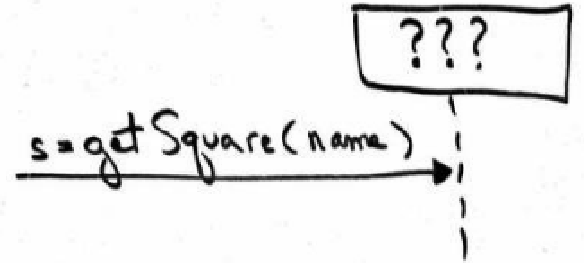
\includegraphics[scale=0.45]{images/Monopoly4.png}
        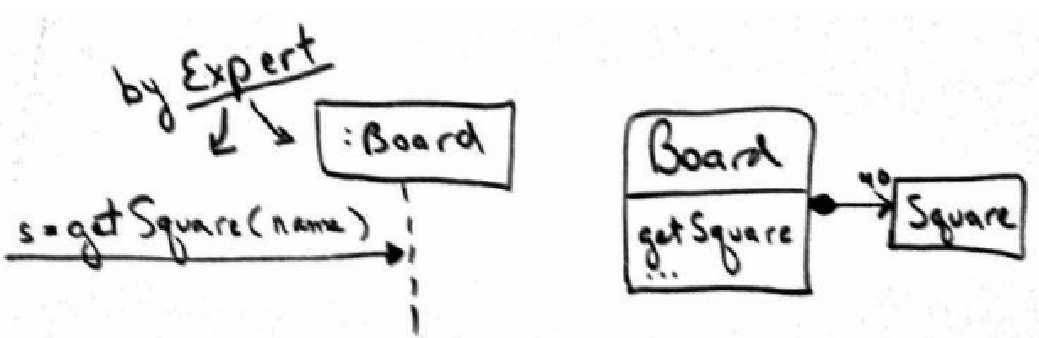
\includegraphics[scale=0.40]{images/Monopoly5.png}
    \end{center}

}

\clm{}{}{
    \begin{itemize}
        \item [$\Rightarrow$] Si individuano informazioni parziali di cui
        diverse classi sono esperte: queste classi possono collaborare
        per soddisfare la responsabilità;
        \item [$\Rightarrow$] Gli oggetti software, a differenza degli oggetti
        \textit{reali}, hanno la responsabilità di compiere azioni sulle cose che conoscono.
    \end{itemize}
}

\subsection{Low Coupling}

\mypattern{Low Coupling - Accoppiamento basso}{
    \paragraph{Problema:} Come ridurre l’impatto dei cambiamenti? Come sostenere una dipendenza
    bassa, un impatto dei cambiamenti basso e una maggiore opportunità di riuso?

    \paragraph{Soluzione:} Assegnare le responsabilità in modo tale che l’accoppiamento (non necessario)
    rimanga basso.
}

\subsection{Controller}

\mypattern{Controller - Controllore}{
    \paragraph{Problema:} Qual è il primo oggetto oltre lo strato UI che riceve e coordina (“controlla”)
    un’operazione di sistema?

    \paragraph{Soluzione:} Assegnare le responsabilità a un oggetto che rappresenta una delle seguenti scelte:
    \begin{itemize}
        \item [$\Rightarrow$] Un oggetto che rappresenta il sistema;
        \item [$\Rightarrow$] Un oggetto che rappresenta uno scenario di un Caso d’Uso.
    \end{itemize}
}

\subsection{High Cohesion - Coesione alta}

\mypattern{High Cohesion}{
    \paragraph{Problema:} Come mantenere gli oggetti focalizzati, comprensibili e gestibili e, come effetto
    collaterale, sostenere Low Coupling?

    \paragraph{Soluzione:} Assegnare le responsabilità in modo tale che la coesione rimanga alta

}

\section{La Progettazione con i pattern GRASP}

\definecolor{chaptergrey}{rgb}{0.21,0.37,0.23}
\ifnum\layout=2 
    \fancyhf{}      
    \renewcommand{\headrulewidth}{0pt}
    \renewcommand{\chaptermark}[1]{\markboth{#1}{}}

    \fancyhead[LE]{\nouppercase{\textbf{\textcolor{chaptergrey}{\chaptername}}~ \thechapter~ |~ \leftmark}}
    \fancyhead[RO]{\nouppercase{ \rightmark}}
    \fancyfoot[LE,RO]{\thepage}
    \fancypagestyle{plain}{         
    \fancyhf{}
    \fancyfoot[LE,RO]{\thepage}}    
 \else          
    \renewcommand{\headrulewidth}{0pt}
    \fancyhf{}                  
    \fancyhead[C]{\nouppercase{ \leftmark}}
    \fancyfoot[C]{\thepage}
\fi

\chapter{Pattern GoF}

\section{Design Pattern GoF}

\section{GoF in Java}

\definecolor{chaptergrey}{rgb}{0.5,0.5,0.5}

\ifnum\layout=2 
    \fancyhf{}      
    \renewcommand{\headrulewidth}{0pt}
    \renewcommand{\chaptermark}[1]{\markboth{#1}{}}

    \fancyhead[LE]{\nouppercase{\textbf{\textcolor{chaptergrey}{\chaptername}}~ \thechapter~ |~ \leftmark}}
    \fancyhead[RO]{\nouppercase{ \rightmark}}
    \fancyfoot[LE,RO]{\thepage}
    \fancypagestyle{plain}{         
    \fancyhf{}
    \fancyfoot[LE,RO]{\thepage}}    
 \else          
    \renewcommand{\headrulewidth}{0pt}
    \fancyhf{}                  
    \fancyhead[C]{\nouppercase{ \leftmark}}
    \fancyfoot[C]{\thepage}
\fi
\chapter{Dal progetto al codice}

\section{Trasformare i progetti in codice}

\section{Sviluppo test-driven e refactoring}

\end{document}